\documentclass[twoside]{book}

% Packages required by doxygen
\usepackage{fixltx2e}
\usepackage{calc}
\usepackage{doxygen}
\usepackage[export]{adjustbox} % also loads graphicx
\usepackage{graphicx}
\usepackage[utf8]{inputenc}
\usepackage{makeidx}
\usepackage{multicol}
\usepackage{multirow}
\PassOptionsToPackage{warn}{textcomp}
\usepackage{textcomp}
\usepackage[nointegrals]{wasysym}
\usepackage[table]{xcolor}

% Font selection
\usepackage[T1]{fontenc}
\usepackage[scaled=.90]{helvet}
\usepackage{courier}
\usepackage{amssymb}
\usepackage{sectsty}
\renewcommand{\familydefault}{\sfdefault}
\allsectionsfont{%
  \fontseries{bc}\selectfont%
  \color{darkgray}%
}
\renewcommand{\DoxyLabelFont}{%
  \fontseries{bc}\selectfont%
  \color{darkgray}%
}
\newcommand{\+}{\discretionary{\mbox{\scriptsize$\hookleftarrow$}}{}{}}

% Page & text layout
\usepackage{geometry}
\geometry{%
  a4paper,%
  top=2.5cm,%
  bottom=2.5cm,%
  left=2.5cm,%
  right=2.5cm%
}
\tolerance=750
\hfuzz=15pt
\hbadness=750
\setlength{\emergencystretch}{15pt}
\setlength{\parindent}{0cm}
\setlength{\parskip}{3ex plus 2ex minus 2ex}
\makeatletter
\renewcommand{\paragraph}{%
  \@startsection{paragraph}{4}{0ex}{-1.0ex}{1.0ex}{%
    \normalfont\normalsize\bfseries\SS@parafont%
  }%
}
\renewcommand{\subparagraph}{%
  \@startsection{subparagraph}{5}{0ex}{-1.0ex}{1.0ex}{%
    \normalfont\normalsize\bfseries\SS@subparafont%
  }%
}
\makeatother

% Headers & footers
\usepackage{fancyhdr}
\pagestyle{fancyplain}
\fancyhead[LE]{\fancyplain{}{\bfseries\thepage}}
\fancyhead[CE]{\fancyplain{}{}}
\fancyhead[RE]{\fancyplain{}{\bfseries\leftmark}}
\fancyhead[LO]{\fancyplain{}{\bfseries\rightmark}}
\fancyhead[CO]{\fancyplain{}{}}
\fancyhead[RO]{\fancyplain{}{\bfseries\thepage}}
\fancyfoot[LE]{\fancyplain{}{}}
\fancyfoot[CE]{\fancyplain{}{}}
\fancyfoot[RE]{\fancyplain{}{\bfseries\scriptsize Generated by Doxygen }}
\fancyfoot[LO]{\fancyplain{}{\bfseries\scriptsize Generated by Doxygen }}
\fancyfoot[CO]{\fancyplain{}{}}
\fancyfoot[RO]{\fancyplain{}{}}
\renewcommand{\footrulewidth}{0.4pt}
\renewcommand{\chaptermark}[1]{%
  \markboth{#1}{}%
}
\renewcommand{\sectionmark}[1]{%
  \markright{\thesection\ #1}%
}

% Indices & bibliography
\usepackage{natbib}
\usepackage[titles]{tocloft}
\setcounter{tocdepth}{3}
\setcounter{secnumdepth}{5}
\makeindex

% Hyperlinks (required, but should be loaded last)
\usepackage{ifpdf}
\ifpdf
  \usepackage[pdftex,pagebackref=true]{hyperref}
\else
  \usepackage[ps2pdf,pagebackref=true]{hyperref}
\fi
\hypersetup{%
  colorlinks=true,%
  linkcolor=blue,%
  citecolor=blue,%
  unicode%
}

% Custom commands
\newcommand{\clearemptydoublepage}{%
  \newpage{\pagestyle{empty}\cleardoublepage}%
}

\usepackage{caption}
\captionsetup{labelsep=space,justification=centering,font={bf},singlelinecheck=off,skip=4pt,position=top}

%===== C O N T E N T S =====

\begin{document}

% Titlepage & ToC
\hypersetup{pageanchor=false,
             bookmarksnumbered=true,
             pdfencoding=unicode
            }
\pagenumbering{roman}
\begin{titlepage}
\vspace*{7cm}
\begin{center}%
{\Large Erriez D\+S3231 high precision I2C R\+TC library for Arduino \\[1ex]\large 1.\+0.\+0 }\\
\vspace*{1cm}
{\large Generated by Doxygen 1.8.11}\\
\end{center}
\end{titlepage}
\clearemptydoublepage
\tableofcontents
\clearemptydoublepage
\pagenumbering{arabic}
\hypersetup{pageanchor=true}

%--- Begin generated contents ---
\chapter{D\+S3231 high precision I2C R\+TC library for Arduino}
\label{index}\hypertarget{index}{}\href{https://travis-ci.org/Erriez/ErriezDS3231}{\tt }

This is an advanced \hyperlink{class_d_s3231}{D\+S3231} high precision I2C R\+TC library for Arduino.



\subsection*{Library features}


\begin{DoxyItemize}
\item Read time
\item Set time
\item Read date and time
\item Set date and time
\item Read Unix Epoch U\+TC 32-\/bit timestamp
\item Read temperature (0.\+25 degree resolution)
\item Alarm 1 (second/minute/hour/day/date match)
\item Alarm 2 (minute/hour/day/date match)
\item Polling and Alarm {\ttfamily I\+N\+T/\+S\+QW} interrupt pin
\item Control {\ttfamily 32k\+Hz} out signal (enable/disable)
\item Control {\ttfamily S\+QW} signal (disable/1/1024/4096/8192\+Hz)
\item Configure aging offset
\item Serial terminal interface
\item Full R\+TC register access
\item Easy debug functionality
\item Basic and advanced examples
\item Set date/time over serial with Python script
\item Low R\+AM footprint\+:
\begin{DoxyItemize}
\item {\ttfamily sizeof(\+D\+S3231)}\+: 1 Byte R\+TC object.
\item {\ttfamily sizeof(\+D\+S3231\+\_\+\+Date\+Time)}\+: 8 Bytes date/time object.
\end{DoxyItemize}
\item Full Doxygen documentation
\end{DoxyItemize}

\subsection*{Hardware}

Any Arduino hardware with a T\+WI interface and {\ttfamily Wire.\+h} support.



\subsection*{Pins}

\tabulinesep=1mm
\begin{longtabu} spread 0pt [c]{*6{|X[-1]}|}
\hline
\rowcolor{\tableheadbgcolor}{\bf Pins board -\/ \hyperlink{class_d_s3231}{D\+S3231} }&\PBS\centering {\bf V\+CC }&\PBS\centering {\bf G\+ND }&\PBS\centering {\bf S\+DA }&\PBS\centering {\bf S\+CL }&\PBS\centering {\bf S\+QW  }\\\cline{1-6}
\endfirsthead
\hline
\endfoot
\hline
\rowcolor{\tableheadbgcolor}{\bf Pins board -\/ \hyperlink{class_d_s3231}{D\+S3231} }&\PBS\centering {\bf V\+CC }&\PBS\centering {\bf G\+ND }&\PBS\centering {\bf S\+DA }&\PBS\centering {\bf S\+CL }&\PBS\centering {\bf S\+QW  }\\\cline{1-6}
\endhead
Arduino U\+NO (A\+T\+Mega328 boards) &\PBS\centering 5V &\PBS\centering G\+ND &\PBS\centering A4 &\PBS\centering A5 &\PBS\centering D2 (I\+N\+T0) \\\cline{1-6}
Arduino Mega2560 &\PBS\centering 5V &\PBS\centering G\+ND &\PBS\centering D20 &\PBS\centering D21 &\PBS\centering D2 (I\+N\+T4) \\\cline{1-6}
Arduino Leonardo &\PBS\centering 5V &\PBS\centering G\+ND &\PBS\centering D2 &\PBS\centering D3 &\PBS\centering D7 (I\+N\+T6) \\\cline{1-6}
Arduino D\+UE (A\+T\+S\+A\+M3\+X8E) &\PBS\centering 3\+V3 &\PBS\centering G\+ND &\PBS\centering 20 &\PBS\centering 21 &\PBS\centering 2 \\\cline{1-6}
E\+S\+P8266 &\PBS\centering 3\+V3 &\PBS\centering G\+ND &\PBS\centering G\+P\+I\+O4 (D2) &\PBS\centering G\+P\+I\+O5 (D1) &\PBS\centering G\+P\+I\+O0 (D3) \\\cline{1-6}
E\+S\+P32 &\PBS\centering 3\+V3 &\PBS\centering G\+ND &\PBS\centering G\+P\+I\+O21 &\PBS\centering G\+P\+I\+O22 &\PBS\centering G\+P\+I\+O0 \\\cline{1-6}
\end{longtabu}
Tested boards\+:


\begin{DoxyItemize}
\item {\bfseries E\+S\+P8266 boards}\+: E\+S\+P12E / We\+Mos D1 \& R2 / Node M\+CU v2 / v3
\item {\bfseries E\+S\+P32 boards\+:} We\+Mos L\+O\+L\+I\+N32 / L\+O\+L\+IN D32
\end{DoxyItemize}

\subsection*{Examples}

Arduino I\+DE $\vert$ Examples $\vert$ Erriez \hyperlink{class_d_s3231}{D\+S3231} R\+TC\+:


\begin{DoxyItemize}
\item \href{https://github.com/Erriez/ErriezDS3231/blob/master/examples/AgingOffset/AgingOffset.ino}{\tt Aging\+Offset} Aging offset programming.
\item \href{https://github.com/Erriez/ErriezDS3231/blob/master/examples/AlarmInterrupt/AlarmInterrupt.ino}{\tt Alarm\+Interrupt} Alarm with interrupts.
\item \href{https://github.com/Erriez/ErriezDS3231/blob/master/examples/AlarmPolling/AlarmPolling.ino}{\tt Alarm\+Polling} Alarm polled.
\item \href{https://github.com/Erriez/ErriezDS3231/blob/master/examples/GettingStarted/GettingStarted.ino}{\tt Getting\+Started} Getting started example which contains most date/time/temperature features.
\item \href{https://github.com/Erriez/ErriezDS3231/blob/master/examples/Minimum/Minimum.ino}{\tt Minimum} Minimum example to read time.
\item \href{https://github.com/Erriez/ErriezDS3231/blob/master/examples/PrintDiagnostics/PrintDiagnostics.ino}{\tt Print\+Diagnostics} Print diagnostics and registers.
\item \href{https://github.com/Erriez/ErriezDS3231/blob/master/examples/ReadTimeInterrupt/ReadTimeInterrupt.ino}{\tt Read\+Time\+Interrupt} Read time with 1\+Hz S\+QW interrupt. (Highly recommended)
\item \href{https://github.com/Erriez/ErriezDS3231/blob/master/examples/ReadTimePolled/ReadTimePolled.ino}{\tt Read\+Time\+Polled} Read time polled.
\item \href{https://github.com/Erriez/ErriezDS3231/blob/master/examples/SetDateTime/SetDateTime.ino}{\tt Set\+Date\+Time} Set date time. (Must be started first)
\item \href{https://github.com/Erriez/ErriezDS3231/blob/master/examples/Temperature/Temperature.ino}{\tt Temperature} Temperature.
\item \href{https://github.com/Erriez/ErriezDS3231/blob/master/examples/Terminal/Terminal.ino}{\tt Terminal} Advanced terminal interface with \href{https://github.com/Erriez/ErriezDS3231/blob/master/examples/Terminal/Terminal.py}{\tt set date/time Python} script.
\end{DoxyItemize}

\subsection*{Documentation}


\begin{DoxyItemize}
\item \href{https://erriez.github.io/ErriezDS3231}{\tt Doxygen online H\+T\+ML}
\item \href{https://github.com/Erriez/ErriezDS3231/raw/gh-pages/latex/ErriezDS3231.pdf}{\tt Doxygen P\+DF}
\item \href{https://github.com/Erriez/ErriezDS3231/blob/master/extras/DS3231.pdf}{\tt D\+S3231 datasheet}
\end{DoxyItemize}

\subsection*{Usage}

{\bfseries Initialization}


\begin{DoxyCode}
1 \{c++\}
2 #include <Wire.h>
3 #include <ErriezDS3231.h>
4 
5 // Create DS3231 RTC object
6 static DS3231 rtc;
7 
8 
9 void setup()
10 \{
11     // Initialize TWI with a 100kHz (default) or 400kHz clock
12     Wire.begin();
13     Wire.setClock(400000);
14 
15     // Initialize RTC
16     while (rtc.begin()) \{
17         // Error: Could not detect DS3231 RTC, retry after some time
18         delay(3000);
19     \}
20 \}
\end{DoxyCode}


{\bfseries Check oscillator status at startup}


\begin{DoxyCode}
1 \{c++\}
2 // Check oscillator status
3 if (rtc.isOscillatorStopped()) \{
4     // Error: DS3231 RTC oscillator stopped. Date/time cannot be trusted. 
5     // Set new date/time before reading date/time.
6     while (1) \{
7         ;
8     \}
9 \}
\end{DoxyCode}


{\bfseries Set time}


\begin{DoxyCode}
1 \{c++\}
2 // Write time to RTC
3 if (rtc.setTime(12, 0, 0)) \{
4     // Error: Write time failed
5 \}
\end{DoxyCode}


{\bfseries Get time}


\begin{DoxyCode}
1 \{c++\}
2 uint8\_t hour;
3 uint8\_t minute;
4 uint8\_t second;
5 
6 // Read time from RTC
7 if (rtc.getTime(&hour, &minute, &second)) \{
8     // Error: Read time failed
9 \}
\end{DoxyCode}


{\bfseries Set date time}


\begin{DoxyCode}
1 \{c++\}
2 // Create and initialize date time object
3 static DS3231\_DateTime dt = \{
4     .second = 0,
5     .minute = 36,
6     .hour = 21,
7     .dayWeek = 7, // 1 = Monday
8     .dayMonth = 29,
9     .month = 7,
10     .year = 2018
11 \};
12 
13 // Set new RTC date/time
14 rtc.setDateTime(&dt);
\end{DoxyCode}


{\bfseries Get date time}


\begin{DoxyCode}
1 \{c++\}
2 DS3231\_DateTime dt;
3 
4 // Read RTC date and time from RTC
5 if (rtc.getDateTime(&dt)) \{
6     // Error: Read date time failed
7 \}
\end{DoxyCode}


{\bfseries Get Epoch Unix U\+TC time}


\begin{DoxyCode}
1 \{c++\}
2 uint32\_t epoch;
3 
4 // Read date/time from RTC
5 if (rtc.getDateTime(&dt)) \{
6     // Error: Read date/time failed
7     return;
8 \}
9 
10 // Convert date/time to 32-bit epoch time
11 epoch = rtc.getEpochTime(&dt));
\end{DoxyCode}


{\bfseries Get temperature}


\begin{DoxyCode}
1 \{c++\}
2 int8\_t temperature;
3 uint8\_t fraction;
4 
5 // Force temperature conversion
6 // Without this call, it takes 64 seconds before the temperature is updated.
7 rtc.startTemperatureConversion();
8 
9 // Read temperature
10 rtc.getTemperature(&temperature, &fraction);
11 
12 // Print temperature. The output below is for example: 28.25C
13 Serial.print(temperature);
14 Serial.print(F("."));
15 Serial.print(fraction);
16 Serial.println(F("C"));
\end{DoxyCode}


{\bfseries Program Alarm 1}

Note\+: Alarm 1 and Alarm 2 have different behavior. Please refer to the documentation which {\ttfamily Alarm1\+Type} and {\ttfamily Alarm2\+Type} are supported. Some examples\+:


\begin{DoxyCode}
1 \{c++\}
2 // Generate alarm 1 every second
3 rtc.setAlarm1(Alarm1EverySecond, 0, 0, 0, 0);
4 
5 // Generate alarm 1 every minute and second match
6 rtc.setAlarm1(Alarm1EverySecond, 0, 0, 45, 30);
7 
8 // Generate alarm 1 every day, hour, minute and second match
9 rtc.setAlarm1(Alarm1MatchDay, 
10               1,  // Alarm day match (1 = Monday)
11               12, // Alarm hour match
12               45, // Alarm minute match
13               30  // Alarm second match
14 );
\end{DoxyCode}


{\bfseries Program Alarm 2}


\begin{DoxyCode}
1 \{c++\}
2 // Generate alarm 2 every minute
3 rtc.setAlarm2(Alarm2EveryMinute, 0, 0, 0);
4 
5 // Generate alarm 2 every hour, minute match
6 rtc.setAlarm2(Alarm2MatchHours, 0, 23, 59);
7 
8 // Generate alarm 2 every date, hour, minute match
9 rtc.setAlarm2(Alarm2MatchDate, 28, 7, 0);
\end{DoxyCode}


{\bfseries Alarm polling}

Note\+: The {\ttfamily I\+NT} pin changes to low when an Alarm 1 or Alarm 2 match occurs and and the interrupt is enabled. The pin remains low until both alarm flags are cleared by the application.


\begin{DoxyCode}
1 \{c++\}
2 // Poll alarm 1 flag
3 if (rtc.getAlarmFlag(Alarm1)) \{
4     // Handle Alarm 1
5 
6     // Clear alarm 1 flag
7     rtc.clearAlarmFlag(Alarm1);
8 \}
9 
10 // Poll alarm 2 flag
11 if (rtc.getAlarmFlag(Alarm2)) \{
12     // Handle Alarm 2
13 
14     // Clear alarm 2 flag
15     rtc.clearAlarmFlag(Alarm2);
16 \}
\end{DoxyCode}


{\bfseries Alarm interrupt}

Note\+: Enabling interrupt will disable the {\ttfamily S\+QW} output signal.


\begin{DoxyCode}
1 \{c++\}
2 // Uno, Nano, Mini, other 328-based: pin D2 (INT0) or D3 (INT1)
3 #define INT\_PIN     2
4 
5 // Alarm interrupt flag must be volatile
6 static volatile bool alarmInterrupt = false;
7 
8 
9 static void alarmHandler()
10 \{
11     // Set global interrupt flag
12     alarmInterrupt = true;
13 \}
14 
15 void setup()
16 \{
17     ...
18 
19     // Attach to INT0 interrupt falling edge
20     pinMode(INT\_PIN, INPUT\_PULLUP);
21     attachInterrupt(digitalPinToInterrupt(INT\_PIN), alarmHandler, FALLING);
22 
23     // Enable Alarm 1 and 2 interrupts
24     rtc.alarmInterruptEnable(Alarm1, true);
25     rtc.alarmInterruptEnable(Alarm2, true);
26 \}
27 
28 void loop()
29 \{
30     // Check global alarm interrupt flag
31     if (alarmInterrupt) \{
32         if (rtc.getAlarmFlag(Alarm1)) \{
33             // Handle alarm 1
34 
35             // Clear alarm 1 interrupt
36             rtc.clearAlarmFlag(Alarm1);
37         \}
38 
39         if (rtc.getAlarmFlag(Alarm2)) \{
40             // Handle alarm 2
41 
42             // Clear alarm 2 interrupt
43             rtc.clearAlarmFlag(Alarm2);
44         \}
45     \}
46 \}
\end{DoxyCode}


{\bfseries 32k\+Hz clock out}

Enable or disable {\ttfamily 32k\+Hz} output pin.


\begin{DoxyCode}
1 \{c++\}
2 rtc.outputClockPinEnable(true);     // Enable 
3 rtc.outputClockPinEnable(false);    // Disable
\end{DoxyCode}


{\bfseries Square Wave Out (S\+QW)}

Note\+: Enabling {\ttfamily S\+QW} pin will disable the alarm {\ttfamily I\+NT} signal.


\begin{DoxyCode}
1 \{c++\}
2 rtc.setSquareWave(SquareWaveDisable);   // Disable
3 rtc.setSquareWave(SquareWave1Hz);       // 1Hz
4 rtc.setSquareWave(SquareWave1024Hz);    // 1024Hz
5 rtc.setSquareWave(SquareWave4096Hz);    // 4096Hz
6 rtc.setSquareWave(SquareWave8192Hz);    // 8192Hz
\end{DoxyCode}


\subsection*{Library dependencies}


\begin{DoxyItemize}
\item {\ttfamily Wire.\+h}
\item {\ttfamily Terminal.\+ino} requires {\ttfamily Erriez\+Serial\+Terminal} library.
\end{DoxyItemize}

\subsection*{Library installation}

Please refer to the \href{https://github.com/Erriez/ErriezArduinoLibrariesAndSketches/wiki}{\tt Wiki} page.

\subsection*{Other Arduino Libraries and Sketches from Erriez}


\begin{DoxyItemize}
\item \href{https://github.com/Erriez/ErriezArduinoLibrariesAndSketches}{\tt Erriez Libraries and Sketches} 
\end{DoxyItemize}
\chapter{Hierarchical Index}
\section{Class Hierarchy}
This inheritance list is sorted roughly, but not completely, alphabetically\+:\begin{DoxyCompactList}
\item \contentsline{section}{D\+S3231}{\pageref{class_d_s3231}}{}
\begin{DoxyCompactList}
\item \contentsline{section}{D\+S3231\+Debug}{\pageref{class_d_s3231_debug}}{}
\end{DoxyCompactList}
\item \contentsline{section}{D\+S3231\+\_\+\+Date\+Time\+\_\+s}{\pageref{struct_d_s3231___date_time__s}}{}
\end{DoxyCompactList}

\chapter{Class Index}
\section{Class List}
Here are the classes, structs, unions and interfaces with brief descriptions\+:\begin{DoxyCompactList}
\item\contentsline{section}{\hyperlink{class_d_s3231}{D\+S3231} \\*\hyperlink{class_d_s3231}{D\+S3231} R\+TC base class }{\pageref{class_d_s3231}}{}
\item\contentsline{section}{\hyperlink{struct_d_s3231___date_time__s}{D\+S3231\+\_\+\+Date\+Time\+\_\+s} \\*Date time structure }{\pageref{struct_d_s3231___date_time__s}}{}
\item\contentsline{section}{\hyperlink{class_d_s3231_debug}{D\+S3231\+Debug} \\*\hyperlink{class_d_s3231}{D\+S3231} R\+TC debug class }{\pageref{class_d_s3231_debug}}{}
\end{DoxyCompactList}

\chapter{File Index}
\section{File List}
Here is a list of all documented files with brief descriptions\+:\begin{DoxyCompactList}
\item\contentsline{section}{\hyperlink{_d_s3231_8cpp}{D\+S3231.\+cpp} \\*\hyperlink{class_d_s3231}{D\+S3231} high precision R\+TC library for Arduino }{\pageref{_d_s3231_8cpp}}{}
\item\contentsline{section}{\hyperlink{_d_s3231_8h}{D\+S3231.\+h} \\*\hyperlink{class_d_s3231}{D\+S3231} high precision R\+TC library for Arduino }{\pageref{_d_s3231_8h}}{}
\item\contentsline{section}{\hyperlink{_d_s3231__debug_8cpp}{D\+S3231\+\_\+debug.\+cpp} \\*\hyperlink{class_d_s3231}{D\+S3231} high precision R\+TC debug library for Arduino }{\pageref{_d_s3231__debug_8cpp}}{}
\item\contentsline{section}{\hyperlink{_d_s3231__debug_8h}{D\+S3231\+\_\+debug.\+h} \\*\hyperlink{class_d_s3231}{D\+S3231} high precision R\+TC debug library for Arduino }{\pageref{_d_s3231__debug_8h}}{}
\end{DoxyCompactList}

\chapter{Class Documentation}
\hypertarget{class_d_s3231}{}\section{D\+S3231 Class Reference}
\label{class_d_s3231}\index{D\+S3231@{D\+S3231}}


\hyperlink{class_d_s3231}{D\+S3231} R\+TC base class.  




{\ttfamily \#include $<$D\+S3231.\+h$>$}

Inheritance diagram for D\+S3231\+:\begin{figure}[H]
\begin{center}
\leavevmode
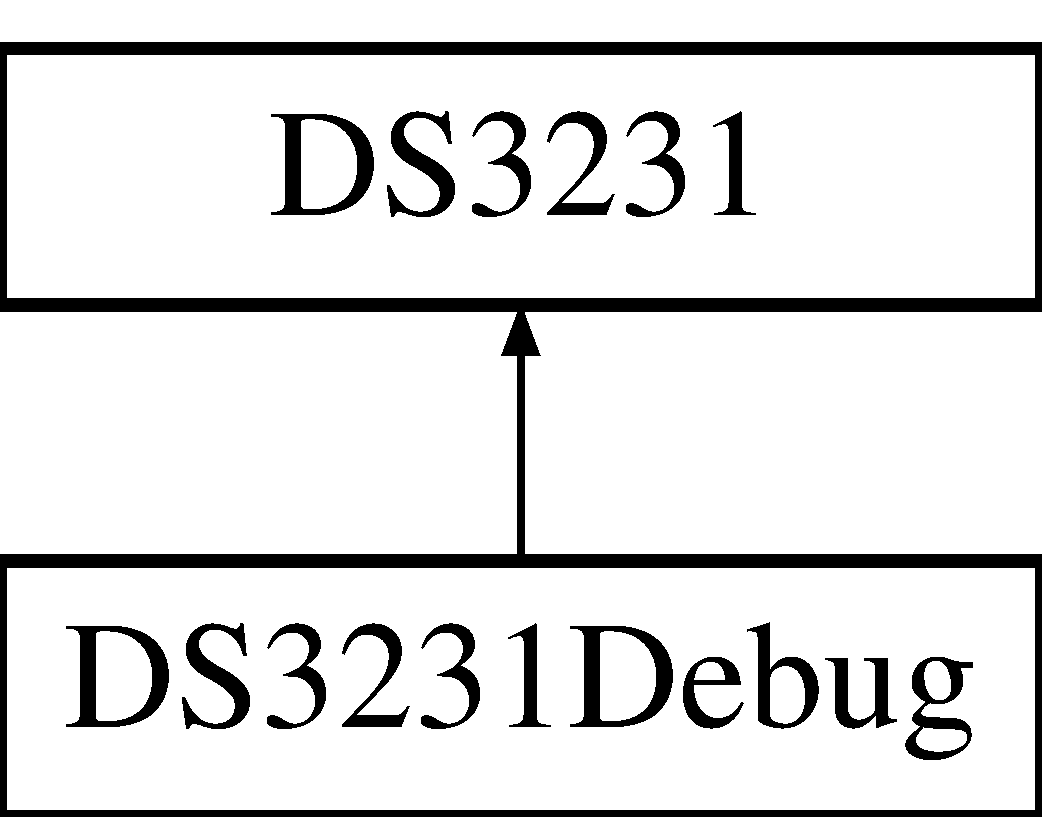
\includegraphics[height=2.000000cm]{class_d_s3231}
\end{center}
\end{figure}
\subsection*{Public Member Functions}
\begin{DoxyCompactItemize}
\item 
bool \hyperlink{class_d_s3231_ac7274a84831c60fe1df1598c47dfb614}{begin} ()
\begin{DoxyCompactList}\small\item\em Initialize and detect \hyperlink{class_d_s3231}{D\+S3231} R\+TC. \end{DoxyCompactList}\item 
void \hyperlink{class_d_s3231_adb2265225b415564a593d8dc5452ba96}{oscillator\+Enable} (bool enable)
\begin{DoxyCompactList}\small\item\em Enable or disable oscillator when running on V-\/\+B\+AT. \end{DoxyCompactList}\item 
bool \hyperlink{class_d_s3231_a1bc59796227778857b5f9978d096b6fd}{is\+Oscillator\+Stopped} ()
\begin{DoxyCompactList}\small\item\em Read R\+TC O\+SF (Oscillator Stop Flag) from status register. \end{DoxyCompactList}\item 
void \hyperlink{class_d_s3231_a380b72e98c720380145039995f22fa0e}{clear\+Oscillator\+Stop\+Flag} ()\hypertarget{class_d_s3231_a380b72e98c720380145039995f22fa0e}{}\label{class_d_s3231_a380b72e98c720380145039995f22fa0e}

\begin{DoxyCompactList}\small\item\em Clear Oscillator Stop Flag (O\+SF) in status register. \end{DoxyCompactList}\item 
void \hyperlink{class_d_s3231_aef50339f978d9fbe4cdd42e38c26fc0c}{set\+Date\+Time} (\hyperlink{_d_s3231_8h_a79a5c1f4b249b6f512ca108013374536}{D\+S3231\+\_\+\+Date\+Time} $\ast$date\+Time)
\begin{DoxyCompactList}\small\item\em Write date and time to R\+TC. \end{DoxyCompactList}\item 
bool \hyperlink{class_d_s3231_a5c627e2a9a7b7c9c99723b6c0916889f}{get\+Date\+Time} (\hyperlink{_d_s3231_8h_a79a5c1f4b249b6f512ca108013374536}{D\+S3231\+\_\+\+Date\+Time} $\ast$date\+Time)
\begin{DoxyCompactList}\small\item\em Read date and time from R\+TC. \end{DoxyCompactList}\item 
void \hyperlink{class_d_s3231_a03ff0537cadf522c98801d42fe55bb08}{set\+Time} (uint8\+\_\+t hour, uint8\+\_\+t minute, uint8\+\_\+t second)
\begin{DoxyCompactList}\small\item\em Write time to R\+TC. \end{DoxyCompactList}\item 
bool \hyperlink{class_d_s3231_ac4b80a2bcda996f2629b2197688d79bc}{get\+Time} (uint8\+\_\+t $\ast$hour, uint8\+\_\+t $\ast$minute, uint8\+\_\+t $\ast$second)
\begin{DoxyCompactList}\small\item\em Read time from R\+TC. \end{DoxyCompactList}\item 
uint32\+\_\+t \hyperlink{class_d_s3231_af0e5a643bf64755c12e40f8cf293035b}{get\+Epoch\+Time} (\hyperlink{_d_s3231_8h_a79a5c1f4b249b6f512ca108013374536}{D\+S3231\+\_\+\+Date\+Time} $\ast$date\+Time)
\begin{DoxyCompactList}\small\item\em Get Unix Epoch 32-\/bit timestamp in current timezone. \end{DoxyCompactList}\item 
void \hyperlink{class_d_s3231_a3386f9c527b7e94ef20338af45b9ba24}{set\+Alarm1} (\hyperlink{_d_s3231_8h_aa29471da8f6d22930cc9159a55a49273}{Alarm1\+Type} alarm\+Type, uint8\+\_\+t day\+Date, uint8\+\_\+t hours, uint8\+\_\+t minutes, uint8\+\_\+t seconds)
\begin{DoxyCompactList}\small\item\em Set Alarm 1. \end{DoxyCompactList}\item 
void \hyperlink{class_d_s3231_a377799172e4f431288e18ff95cf5b7ec}{set\+Alarm2} (\hyperlink{_d_s3231_8h_a2561c628950a85b8f502b7055c3acd8b}{Alarm2\+Type} alarm\+Type, uint8\+\_\+t day\+Date, uint8\+\_\+t hours, uint8\+\_\+t minutes)
\begin{DoxyCompactList}\small\item\em Set Alarm 2. \end{DoxyCompactList}\item 
void \hyperlink{class_d_s3231_a0bcf130e164ba5436a71dbb81621fb35}{alarm\+Interrupt\+Enable} (\hyperlink{_d_s3231_8h_abdac868b647b120d540abd60d35e0feb}{Alarm\+Id} alarm\+Id, bool enable)
\begin{DoxyCompactList}\small\item\em Enable or disable Alarm 1 or 2 interrupt. \end{DoxyCompactList}\item 
bool \hyperlink{class_d_s3231_a77104765708a5f7ab9fbec7c17e145ea}{get\+Alarm\+Flag} (\hyperlink{_d_s3231_8h_abdac868b647b120d540abd60d35e0feb}{Alarm\+Id} alarm\+Id)
\begin{DoxyCompactList}\small\item\em Get Alarm 1 or 2 flag. \end{DoxyCompactList}\item 
void \hyperlink{class_d_s3231_ae70cc93049001d830b926491698fdfb6}{clear\+Alarm\+Flag} (\hyperlink{_d_s3231_8h_abdac868b647b120d540abd60d35e0feb}{Alarm\+Id} alarm\+Id)
\begin{DoxyCompactList}\small\item\em Clear alarm flag. \end{DoxyCompactList}\item 
void \hyperlink{class_d_s3231_a9d5ef58a83a5bde590bf414be67fb4a5}{set\+Square\+Wave} (\hyperlink{_d_s3231_8h_aa45f48b2c6f58f91a278a1601b211140}{Square\+Wave} square\+Wave)
\begin{DoxyCompactList}\small\item\em Configure S\+QW (Square Wave) output pin. \end{DoxyCompactList}\item 
void \hyperlink{class_d_s3231_a345592e12ccf5fc6c887c1414f8a3abb}{output\+Clock\+Pin\+Enable} (bool enable)
\begin{DoxyCompactList}\small\item\em Enable or disable 32k\+Hz output clock pin. \end{DoxyCompactList}\item 
void \hyperlink{class_d_s3231_a18f8f98c3d1e8c6fdb611cbb97bbdee0}{set\+Aging\+Offset} (int8\+\_\+t val)
\begin{DoxyCompactList}\small\item\em Set aging offset register. \end{DoxyCompactList}\item 
int8\+\_\+t \hyperlink{class_d_s3231_a4ef9862e078068b915285cd264584449}{get\+Aging\+Offset} ()
\begin{DoxyCompactList}\small\item\em Get aging offset register. \end{DoxyCompactList}\item 
void \hyperlink{class_d_s3231_ad2b2d423930fca422dbc6adfd2a8e571}{start\+Temperature\+Conversion} ()
\begin{DoxyCompactList}\small\item\em Start temperature conversion. \end{DoxyCompactList}\item 
void \hyperlink{class_d_s3231_a334f37eca94eb3cd7d2c780e8268864c}{get\+Temperature} (int8\+\_\+t $\ast$temperature, uint8\+\_\+t $\ast$fraction)
\begin{DoxyCompactList}\small\item\em Read temperature. \end{DoxyCompactList}\item 
uint8\+\_\+t \hyperlink{class_d_s3231_aa49b293f3fdcc222e0f86cc2bbdf1476}{bcd\+To\+Dec} (uint8\+\_\+t bcd)
\begin{DoxyCompactList}\small\item\em B\+CD to decimal conversion. \end{DoxyCompactList}\item 
uint8\+\_\+t \hyperlink{class_d_s3231_a8883c7df954dc7682a40825790631230}{dec\+To\+Bcd} (uint8\+\_\+t dec)
\begin{DoxyCompactList}\small\item\em Decimal to B\+CD conversion. \end{DoxyCompactList}\item 
uint8\+\_\+t \hyperlink{class_d_s3231_a53ae4553629d91e3ab06c22d03fe09e2}{read\+Control\+Register} ()
\begin{DoxyCompactList}\small\item\em Read control register. \end{DoxyCompactList}\item 
void \hyperlink{class_d_s3231_a563f7fd8e44c26f6bd0b035ad9852caa}{write\+Control\+Register} (uint8\+\_\+t value)
\begin{DoxyCompactList}\small\item\em Write control register. \end{DoxyCompactList}\item 
uint8\+\_\+t \hyperlink{class_d_s3231_a29fb8f2fe94a93b80336b183d5e9fc0c}{read\+Status\+Register} ()
\begin{DoxyCompactList}\small\item\em Read status register. \end{DoxyCompactList}\item 
void \hyperlink{class_d_s3231_a5a937c59828e7aef61af8ae8f02bb0f8}{write\+Status\+Register} (uint8\+\_\+t value)
\begin{DoxyCompactList}\small\item\em Write status register. \end{DoxyCompactList}\item 
uint8\+\_\+t \hyperlink{class_d_s3231_a37cac2a6bbf52b801dcaf6471d4418ac}{read\+Register} (uint8\+\_\+t reg)
\begin{DoxyCompactList}\small\item\em Read register. \end{DoxyCompactList}\item 
void \hyperlink{class_d_s3231_a292109841c55ecebb7a920c6f87f5ac5}{write\+Register} (uint8\+\_\+t reg, uint8\+\_\+t value)
\begin{DoxyCompactList}\small\item\em Write to R\+TC register. \end{DoxyCompactList}\item 
void \hyperlink{class_d_s3231_ae72bc3b3e8164477762d14e7961daff0}{read\+Buffer} (uint8\+\_\+t reg, void $\ast$buffer, uint8\+\_\+t len)
\begin{DoxyCompactList}\small\item\em Read buffer from R\+TC. \end{DoxyCompactList}\item 
void \hyperlink{class_d_s3231_a6ba3dae2a1de95f8aaaed331ca47b239}{write\+Buffer} (uint8\+\_\+t reg, void $\ast$buffer, uint8\+\_\+t len)
\begin{DoxyCompactList}\small\item\em Write buffer to R\+TC. \end{DoxyCompactList}\end{DoxyCompactItemize}


\subsection{Detailed Description}
\hyperlink{class_d_s3231}{D\+S3231} R\+TC base class. 

Definition at line 161 of file D\+S3231.\+h.



\subsection{Member Function Documentation}
\index{D\+S3231@{D\+S3231}!alarm\+Interrupt\+Enable@{alarm\+Interrupt\+Enable}}
\index{alarm\+Interrupt\+Enable@{alarm\+Interrupt\+Enable}!D\+S3231@{D\+S3231}}
\subsubsection[{\texorpdfstring{alarm\+Interrupt\+Enable(\+Alarm\+Id alarm\+Id, bool enable)}{alarmInterruptEnable(AlarmId alarmId, bool enable)}}]{\setlength{\rightskip}{0pt plus 5cm}void D\+S3231\+::alarm\+Interrupt\+Enable (
\begin{DoxyParamCaption}
\item[{{\bf Alarm\+Id}}]{alarm\+Id, }
\item[{bool}]{enable}
\end{DoxyParamCaption}
)}\hypertarget{class_d_s3231_a0bcf130e164ba5436a71dbb81621fb35}{}\label{class_d_s3231_a0bcf130e164ba5436a71dbb81621fb35}


Enable or disable Alarm 1 or 2 interrupt. 

Enabling the alarm interrupt will disable the Square Wave output on the I\+N\+T/\+S\+QW pin. The I\+NT pin remains high until an alarm match occurs. 
\begin{DoxyParams}{Parameters}
{\em alarm\+Id} & Alarm1 or Alarm2 enum. \\
\hline
{\em enable} & true\+: Enable alarm interrupt.~\newline
 false\+: Disable alarm interrupt. \\
\hline
\end{DoxyParams}


Definition at line 417 of file D\+S3231.\+cpp.

\index{D\+S3231@{D\+S3231}!bcd\+To\+Dec@{bcd\+To\+Dec}}
\index{bcd\+To\+Dec@{bcd\+To\+Dec}!D\+S3231@{D\+S3231}}
\subsubsection[{\texorpdfstring{bcd\+To\+Dec(uint8\+\_\+t bcd)}{bcdToDec(uint8_t bcd)}}]{\setlength{\rightskip}{0pt plus 5cm}uint8\+\_\+t D\+S3231\+::bcd\+To\+Dec (
\begin{DoxyParamCaption}
\item[{uint8\+\_\+t}]{bcd}
\end{DoxyParamCaption}
)}\hypertarget{class_d_s3231_aa49b293f3fdcc222e0f86cc2bbdf1476}{}\label{class_d_s3231_aa49b293f3fdcc222e0f86cc2bbdf1476}


B\+CD to decimal conversion. 


\begin{DoxyParams}{Parameters}
{\em bcd} & B\+CD encoded value. \\
\hline
\end{DoxyParams}
\begin{DoxyReturn}{Returns}
Decimal value. 
\end{DoxyReturn}


Definition at line 658 of file D\+S3231.\+cpp.

\index{D\+S3231@{D\+S3231}!begin@{begin}}
\index{begin@{begin}!D\+S3231@{D\+S3231}}
\subsubsection[{\texorpdfstring{begin()}{begin()}}]{\setlength{\rightskip}{0pt plus 5cm}bool D\+S3231\+::begin (
\begin{DoxyParamCaption}
{}
\end{DoxyParamCaption}
)}\hypertarget{class_d_s3231_ac7274a84831c60fe1df1598c47dfb614}{}\label{class_d_s3231_ac7274a84831c60fe1df1598c47dfb614}


Initialize and detect \hyperlink{class_d_s3231}{D\+S3231} R\+TC. 

Call this function from setup(). 
\begin{DoxyRetVals}{Return values}
{\em Success} & R\+TC detected. \\
\hline
{\em false} & R\+TC not detected. \\
\hline
{\em true} & Invalid status register or R\+TC not detected. \\
\hline
\end{DoxyRetVals}


Definition at line 55 of file D\+S3231.\+cpp.

\index{D\+S3231@{D\+S3231}!clear\+Alarm\+Flag@{clear\+Alarm\+Flag}}
\index{clear\+Alarm\+Flag@{clear\+Alarm\+Flag}!D\+S3231@{D\+S3231}}
\subsubsection[{\texorpdfstring{clear\+Alarm\+Flag(\+Alarm\+Id alarm\+Id)}{clearAlarmFlag(AlarmId alarmId)}}]{\setlength{\rightskip}{0pt plus 5cm}void D\+S3231\+::clear\+Alarm\+Flag (
\begin{DoxyParamCaption}
\item[{{\bf Alarm\+Id}}]{alarm\+Id}
\end{DoxyParamCaption}
)}\hypertarget{class_d_s3231_ae70cc93049001d830b926491698fdfb6}{}\label{class_d_s3231_ae70cc93049001d830b926491698fdfb6}


Clear alarm flag. 

This function should be called when the alarm flag has been handled in polling and interrupt mode. The I\+NT pin changes to high when both alarm flags are cleared and alarm interrupts are enabled. 
\begin{DoxyParams}{Parameters}
{\em alarm\+Id} & Alarm1 or Alarm2 enum. \\
\hline
\end{DoxyParams}

\begin{DoxyRetVals}{Return values}
{\em Success} & \\
\hline
{\em Failure} & Incorrect alarm ID. \\
\hline
\end{DoxyRetVals}


Definition at line 478 of file D\+S3231.\+cpp.

\index{D\+S3231@{D\+S3231}!dec\+To\+Bcd@{dec\+To\+Bcd}}
\index{dec\+To\+Bcd@{dec\+To\+Bcd}!D\+S3231@{D\+S3231}}
\subsubsection[{\texorpdfstring{dec\+To\+Bcd(uint8\+\_\+t dec)}{decToBcd(uint8_t dec)}}]{\setlength{\rightskip}{0pt plus 5cm}uint8\+\_\+t D\+S3231\+::dec\+To\+Bcd (
\begin{DoxyParamCaption}
\item[{uint8\+\_\+t}]{dec}
\end{DoxyParamCaption}
)}\hypertarget{class_d_s3231_a8883c7df954dc7682a40825790631230}{}\label{class_d_s3231_a8883c7df954dc7682a40825790631230}


Decimal to B\+CD conversion. 


\begin{DoxyParams}{Parameters}
{\em dec} & Decimal value. \\
\hline
\end{DoxyParams}
\begin{DoxyReturn}{Returns}
B\+CD encoded value. 
\end{DoxyReturn}


Definition at line 670 of file D\+S3231.\+cpp.

\index{D\+S3231@{D\+S3231}!get\+Aging\+Offset@{get\+Aging\+Offset}}
\index{get\+Aging\+Offset@{get\+Aging\+Offset}!D\+S3231@{D\+S3231}}
\subsubsection[{\texorpdfstring{get\+Aging\+Offset()}{getAgingOffset()}}]{\setlength{\rightskip}{0pt plus 5cm}int8\+\_\+t D\+S3231\+::get\+Aging\+Offset (
\begin{DoxyParamCaption}
{}
\end{DoxyParamCaption}
)}\hypertarget{class_d_s3231_a4ef9862e078068b915285cd264584449}{}\label{class_d_s3231_a4ef9862e078068b915285cd264584449}


Get aging offset register. 

The aging offset register capacitance value is added or subtracted from the capacitance value that the device calculates for each temperature compensation. \begin{DoxyReturn}{Returns}
val Aging offset value. 
\end{DoxyReturn}


Definition at line 583 of file D\+S3231.\+cpp.

\index{D\+S3231@{D\+S3231}!get\+Alarm\+Flag@{get\+Alarm\+Flag}}
\index{get\+Alarm\+Flag@{get\+Alarm\+Flag}!D\+S3231@{D\+S3231}}
\subsubsection[{\texorpdfstring{get\+Alarm\+Flag(\+Alarm\+Id alarm\+Id)}{getAlarmFlag(AlarmId alarmId)}}]{\setlength{\rightskip}{0pt plus 5cm}bool D\+S3231\+::get\+Alarm\+Flag (
\begin{DoxyParamCaption}
\item[{{\bf Alarm\+Id}}]{alarm\+Id}
\end{DoxyParamCaption}
)}\hypertarget{class_d_s3231_a77104765708a5f7ab9fbec7c17e145ea}{}\label{class_d_s3231_a77104765708a5f7ab9fbec7c17e145ea}


Get Alarm 1 or 2 flag. 

Call this function to retrieve the alarm status flag. This function can be used in polling as well as with interrupts enabled.

The I\+NT pin changes to low when an Alarm 1 or Alarm 2 match occurs and the interrupt is enabled. The pin remains low until both alarm flags are cleared by the application. 
\begin{DoxyParams}{Parameters}
{\em alarm\+Id} & Alarm1 or Alarm2 enum. \\
\hline
\end{DoxyParams}

\begin{DoxyRetVals}{Return values}
{\em true} & Alarm interrupt flag set. \\
\hline
{\em false} & Alarm interrupt flag cleared. \\
\hline
\end{DoxyRetVals}


Definition at line 456 of file D\+S3231.\+cpp.

\index{D\+S3231@{D\+S3231}!get\+Date\+Time@{get\+Date\+Time}}
\index{get\+Date\+Time@{get\+Date\+Time}!D\+S3231@{D\+S3231}}
\subsubsection[{\texorpdfstring{get\+Date\+Time(\+D\+S3231\+\_\+\+Date\+Time $\ast$date\+Time)}{getDateTime(DS3231_DateTime *dateTime)}}]{\setlength{\rightskip}{0pt plus 5cm}bool D\+S3231\+::get\+Date\+Time (
\begin{DoxyParamCaption}
\item[{{\bf D\+S3231\+\_\+\+Date\+Time} $\ast$}]{date\+Time}
\end{DoxyParamCaption}
)}\hypertarget{class_d_s3231_a5c627e2a9a7b7c9c99723b6c0916889f}{}\label{class_d_s3231_a5c627e2a9a7b7c9c99723b6c0916889f}


Read date and time from R\+TC. 

Read all R\+TC registers at once to prevent a time/date register change in the middle of the register read operation. 
\begin{DoxyParams}{Parameters}
{\em date\+Time} & Date and time structure. \\
\hline
\end{DoxyParams}

\begin{DoxyRetVals}{Return values}
{\em false} & Success \\
\hline
{\em true} & An invalid date/time format was read from the R\+TC. \\
\hline
\end{DoxyRetVals}


Definition at line 176 of file D\+S3231.\+cpp.

\index{D\+S3231@{D\+S3231}!get\+Epoch\+Time@{get\+Epoch\+Time}}
\index{get\+Epoch\+Time@{get\+Epoch\+Time}!D\+S3231@{D\+S3231}}
\subsubsection[{\texorpdfstring{get\+Epoch\+Time(\+D\+S3231\+\_\+\+Date\+Time $\ast$date\+Time)}{getEpochTime(DS3231_DateTime *dateTime)}}]{\setlength{\rightskip}{0pt plus 5cm}uint32\+\_\+t D\+S3231\+::get\+Epoch\+Time (
\begin{DoxyParamCaption}
\item[{{\bf D\+S3231\+\_\+\+Date\+Time} $\ast$}]{date\+Time}
\end{DoxyParamCaption}
)}\hypertarget{class_d_s3231_af0e5a643bf64755c12e40f8cf293035b}{}\label{class_d_s3231_af0e5a643bf64755c12e40f8cf293035b}


Get Unix Epoch 32-\/bit timestamp in current timezone. 

The \hyperlink{class_d_s3231}{D\+S3231} R\+TC year range is valid between years 2000...2100. The time is in U\+TC. 
\begin{DoxyRetVals}{Return values}
{\em epoch} & 32-\/bit unsigned Unix Epoch time \\
\hline
\end{DoxyRetVals}


Definition at line 284 of file D\+S3231.\+cpp.

\index{D\+S3231@{D\+S3231}!get\+Temperature@{get\+Temperature}}
\index{get\+Temperature@{get\+Temperature}!D\+S3231@{D\+S3231}}
\subsubsection[{\texorpdfstring{get\+Temperature(int8\+\_\+t $\ast$temperature, uint8\+\_\+t $\ast$fraction)}{getTemperature(int8_t *temperature, uint8_t *fraction)}}]{\setlength{\rightskip}{0pt plus 5cm}void D\+S3231\+::get\+Temperature (
\begin{DoxyParamCaption}
\item[{int8\+\_\+t $\ast$}]{temperature, }
\item[{uint8\+\_\+t $\ast$}]{fraction}
\end{DoxyParamCaption}
)}\hypertarget{class_d_s3231_a334f37eca94eb3cd7d2c780e8268864c}{}\label{class_d_s3231_a334f37eca94eb3cd7d2c780e8268864c}


Read temperature. 


\begin{DoxyParams}{Parameters}
{\em temperature} & 8-\/bit signed temperature in degree Celsius. \\
\hline
{\em fraction} & Temperature fraction in steps of 0.\+25 degree Celsius. The returned value is a decimal value to prevent floating point usage. The application should divided the fraction by 100. \\
\hline
\end{DoxyParams}


Definition at line 630 of file D\+S3231.\+cpp.

\index{D\+S3231@{D\+S3231}!get\+Time@{get\+Time}}
\index{get\+Time@{get\+Time}!D\+S3231@{D\+S3231}}
\subsubsection[{\texorpdfstring{get\+Time(uint8\+\_\+t $\ast$hour, uint8\+\_\+t $\ast$minute, uint8\+\_\+t $\ast$second)}{getTime(uint8_t *hour, uint8_t *minute, uint8_t *second)}}]{\setlength{\rightskip}{0pt plus 5cm}bool D\+S3231\+::get\+Time (
\begin{DoxyParamCaption}
\item[{uint8\+\_\+t $\ast$}]{hour, }
\item[{uint8\+\_\+t $\ast$}]{minute, }
\item[{uint8\+\_\+t $\ast$}]{second}
\end{DoxyParamCaption}
)}\hypertarget{class_d_s3231_ac4b80a2bcda996f2629b2197688d79bc}{}\label{class_d_s3231_ac4b80a2bcda996f2629b2197688d79bc}


Read time from R\+TC. 

Read hour, minute and second registers from R\+TC. 
\begin{DoxyParams}{Parameters}
{\em hour} & Hours 0..23. \\
\hline
{\em minute} & Minutes 0..59. \\
\hline
{\em second} & Seconds 0..59. \\
\hline
\end{DoxyParams}

\begin{DoxyRetVals}{Return values}
{\em false} & Success \\
\hline
{\em true} & Invalid second, minute or hour read from R\+TC. The time is set to zero. \\
\hline
\end{DoxyRetVals}


Definition at line 246 of file D\+S3231.\+cpp.

\index{D\+S3231@{D\+S3231}!is\+Oscillator\+Stopped@{is\+Oscillator\+Stopped}}
\index{is\+Oscillator\+Stopped@{is\+Oscillator\+Stopped}!D\+S3231@{D\+S3231}}
\subsubsection[{\texorpdfstring{is\+Oscillator\+Stopped()}{isOscillatorStopped()}}]{\setlength{\rightskip}{0pt plus 5cm}bool D\+S3231\+::is\+Oscillator\+Stopped (
\begin{DoxyParamCaption}
{}
\end{DoxyParamCaption}
)}\hypertarget{class_d_s3231_a1bc59796227778857b5f9978d096b6fd}{}\label{class_d_s3231_a1bc59796227778857b5f9978d096b6fd}


Read R\+TC O\+SF (Oscillator Stop Flag) from status register. 

The application is responsible for checking the Oscillator Stop Flag (O\+SF) before reading date/time date. This function may be used to judge the validity of the date/time registers. 
\begin{DoxyRetVals}{Return values}
{\em true} & R\+TC oscillator was stopped\+: The date/time data is invalid. The application should synchronize and program a new date/time. \\
\hline
{\em false} & R\+TC oscillator is running. \\
\hline
\end{DoxyRetVals}


Definition at line 104 of file D\+S3231.\+cpp.

\index{D\+S3231@{D\+S3231}!oscillator\+Enable@{oscillator\+Enable}}
\index{oscillator\+Enable@{oscillator\+Enable}!D\+S3231@{D\+S3231}}
\subsubsection[{\texorpdfstring{oscillator\+Enable(bool enable)}{oscillatorEnable(bool enable)}}]{\setlength{\rightskip}{0pt plus 5cm}void D\+S3231\+::oscillator\+Enable (
\begin{DoxyParamCaption}
\item[{bool}]{enable}
\end{DoxyParamCaption}
)}\hypertarget{class_d_s3231_adb2265225b415564a593d8dc5452ba96}{}\label{class_d_s3231_adb2265225b415564a593d8dc5452ba96}


Enable or disable oscillator when running on V-\/\+B\+AT. 


\begin{DoxyParams}{Parameters}
{\em enable} & true\+: Enable R\+TC clock when running on V-\/\+B\+AT.~\newline
 false\+: Stop R\+TC clock when running on V-\/\+B\+AT. Oscillator Stop Flag (O\+SF) bit will be set in status register which can be read on next power-\/on. \\
\hline
\end{DoxyParams}


Definition at line 73 of file D\+S3231.\+cpp.

\index{D\+S3231@{D\+S3231}!output\+Clock\+Pin\+Enable@{output\+Clock\+Pin\+Enable}}
\index{output\+Clock\+Pin\+Enable@{output\+Clock\+Pin\+Enable}!D\+S3231@{D\+S3231}}
\subsubsection[{\texorpdfstring{output\+Clock\+Pin\+Enable(bool enable)}{outputClockPinEnable(bool enable)}}]{\setlength{\rightskip}{0pt plus 5cm}void D\+S3231\+::output\+Clock\+Pin\+Enable (
\begin{DoxyParamCaption}
\item[{bool}]{enable}
\end{DoxyParamCaption}
)}\hypertarget{class_d_s3231_a345592e12ccf5fc6c887c1414f8a3abb}{}\label{class_d_s3231_a345592e12ccf5fc6c887c1414f8a3abb}


Enable or disable 32k\+Hz output clock pin. 


\begin{DoxyParams}{Parameters}
{\em enable} & true\+: Enable 32k\+Hz output clock pin.~\newline
 false\+: Disable 32k\+Hz output clock pin. \\
\hline
\end{DoxyParams}


Definition at line 528 of file D\+S3231.\+cpp.

\index{D\+S3231@{D\+S3231}!read\+Buffer@{read\+Buffer}}
\index{read\+Buffer@{read\+Buffer}!D\+S3231@{D\+S3231}}
\subsubsection[{\texorpdfstring{read\+Buffer(uint8\+\_\+t reg, void $\ast$buffer, uint8\+\_\+t len)}{readBuffer(uint8_t reg, void *buffer, uint8_t len)}}]{\setlength{\rightskip}{0pt plus 5cm}void D\+S3231\+::read\+Buffer (
\begin{DoxyParamCaption}
\item[{uint8\+\_\+t}]{reg, }
\item[{void $\ast$}]{buffer, }
\item[{uint8\+\_\+t}]{len}
\end{DoxyParamCaption}
)}\hypertarget{class_d_s3231_ae72bc3b3e8164477762d14e7961daff0}{}\label{class_d_s3231_ae72bc3b3e8164477762d14e7961daff0}


Read buffer from R\+TC. 


\begin{DoxyParams}{Parameters}
{\em reg} & R\+TC register number 0x00..0x12. \\
\hline
{\em buffer} & Buffer. \\
\hline
{\em len} & Buffer length. Reading is only allowed within valid R\+TC registers. \\
\hline
\end{DoxyParams}


Definition at line 777 of file D\+S3231.\+cpp.

\index{D\+S3231@{D\+S3231}!read\+Control\+Register@{read\+Control\+Register}}
\index{read\+Control\+Register@{read\+Control\+Register}!D\+S3231@{D\+S3231}}
\subsubsection[{\texorpdfstring{read\+Control\+Register()}{readControlRegister()}}]{\setlength{\rightskip}{0pt plus 5cm}uint8\+\_\+t D\+S3231\+::read\+Control\+Register (
\begin{DoxyParamCaption}
{}
\end{DoxyParamCaption}
)}\hypertarget{class_d_s3231_a53ae4553629d91e3ab06c22d03fe09e2}{}\label{class_d_s3231_a53ae4553629d91e3ab06c22d03fe09e2}


Read control register. 

\begin{DoxyReturn}{Returns}
8-\/bit unsigned register value 
\end{DoxyReturn}


Definition at line 680 of file D\+S3231.\+cpp.

\index{D\+S3231@{D\+S3231}!read\+Register@{read\+Register}}
\index{read\+Register@{read\+Register}!D\+S3231@{D\+S3231}}
\subsubsection[{\texorpdfstring{read\+Register(uint8\+\_\+t reg)}{readRegister(uint8_t reg)}}]{\setlength{\rightskip}{0pt plus 5cm}uint8\+\_\+t D\+S3231\+::read\+Register (
\begin{DoxyParamCaption}
\item[{uint8\+\_\+t}]{reg}
\end{DoxyParamCaption}
)}\hypertarget{class_d_s3231_a37cac2a6bbf52b801dcaf6471d4418ac}{}\label{class_d_s3231_a37cac2a6bbf52b801dcaf6471d4418ac}


Read register. 

Please refer to the R\+TC datasheet. 
\begin{DoxyParams}{Parameters}
{\em reg} & R\+TC register number 0x00..0x12. \\
\hline
\end{DoxyParams}
\begin{DoxyReturn}{Returns}
value 8-\/bit unsigned register value. 
\end{DoxyReturn}


Definition at line 721 of file D\+S3231.\+cpp.

\index{D\+S3231@{D\+S3231}!read\+Status\+Register@{read\+Status\+Register}}
\index{read\+Status\+Register@{read\+Status\+Register}!D\+S3231@{D\+S3231}}
\subsubsection[{\texorpdfstring{read\+Status\+Register()}{readStatusRegister()}}]{\setlength{\rightskip}{0pt plus 5cm}uint8\+\_\+t D\+S3231\+::read\+Status\+Register (
\begin{DoxyParamCaption}
{}
\end{DoxyParamCaption}
)}\hypertarget{class_d_s3231_a29fb8f2fe94a93b80336b183d5e9fc0c}{}\label{class_d_s3231_a29fb8f2fe94a93b80336b183d5e9fc0c}


Read status register. 

\begin{DoxyReturn}{Returns}
8-\/bit unsigned register value 
\end{DoxyReturn}


Definition at line 698 of file D\+S3231.\+cpp.

\index{D\+S3231@{D\+S3231}!set\+Aging\+Offset@{set\+Aging\+Offset}}
\index{set\+Aging\+Offset@{set\+Aging\+Offset}!D\+S3231@{D\+S3231}}
\subsubsection[{\texorpdfstring{set\+Aging\+Offset(int8\+\_\+t val)}{setAgingOffset(int8_t val)}}]{\setlength{\rightskip}{0pt plus 5cm}void D\+S3231\+::set\+Aging\+Offset (
\begin{DoxyParamCaption}
\item[{int8\+\_\+t}]{val}
\end{DoxyParamCaption}
)}\hypertarget{class_d_s3231_a18f8f98c3d1e8c6fdb611cbb97bbdee0}{}\label{class_d_s3231_a18f8f98c3d1e8c6fdb611cbb97bbdee0}


Set aging offset register. 

The aging offset register capacitance value is added or subtracted from the capacitance value that the device calculates for each temperature compensation. 
\begin{DoxyParams}{Parameters}
{\em val} & Aging offset value -\/127..127, 0.\+1ppm per L\+SB (Factory default value\+: 0).~\newline
 Negative values increases the R\+TC oscillator frequency. \\
\hline
\end{DoxyParams}


Definition at line 555 of file D\+S3231.\+cpp.

\index{D\+S3231@{D\+S3231}!set\+Alarm1@{set\+Alarm1}}
\index{set\+Alarm1@{set\+Alarm1}!D\+S3231@{D\+S3231}}
\subsubsection[{\texorpdfstring{set\+Alarm1(\+Alarm1\+Type alarm\+Type, uint8\+\_\+t day\+Date, uint8\+\_\+t hours, uint8\+\_\+t minutes, uint8\+\_\+t seconds)}{setAlarm1(Alarm1Type alarmType, uint8_t dayDate, uint8_t hours, uint8_t minutes, uint8_t seconds)}}]{\setlength{\rightskip}{0pt plus 5cm}void D\+S3231\+::set\+Alarm1 (
\begin{DoxyParamCaption}
\item[{{\bf Alarm1\+Type}}]{alarm\+Type, }
\item[{uint8\+\_\+t}]{day\+Date, }
\item[{uint8\+\_\+t}]{hours, }
\item[{uint8\+\_\+t}]{minutes, }
\item[{uint8\+\_\+t}]{seconds}
\end{DoxyParamCaption}
)}\hypertarget{class_d_s3231_a3386f9c527b7e94ef20338af45b9ba24}{}\label{class_d_s3231_a3386f9c527b7e94ef20338af45b9ba24}


Set Alarm 1. 

Alarm 1 contains several alarm modes which can be configured with the alarm\+Type parameter. Unused matches can be set to zero. The alarm interrupt must be enabled after setting the alarm, followed by clearing the alarm interrupt flag. 
\begin{DoxyParams}{Parameters}
{\em alarm\+Type} & Alarm 1 types\+:~\newline
 Alarm1\+Every\+Second~\newline
 Alarm1\+Match\+Seconds~\newline
 Alarm1\+Match\+Minutes~\newline
 Alarm1\+Match\+Hours~\newline
 Alarm1\+Match\+Day~\newline
 Alarm1\+Match\+Date~\newline
\\
\hline
{\em day\+Date} & Alarm match day of the week or day of the month. This depends on alarm\+Type. \\
\hline
{\em hours} & Alarm match hours. \\
\hline
{\em minutes} & Alarm match minutes. \\
\hline
{\em seconds} & Alarm match seconds. \\
\hline
\end{DoxyParams}


Definition at line 339 of file D\+S3231.\+cpp.

\index{D\+S3231@{D\+S3231}!set\+Alarm2@{set\+Alarm2}}
\index{set\+Alarm2@{set\+Alarm2}!D\+S3231@{D\+S3231}}
\subsubsection[{\texorpdfstring{set\+Alarm2(\+Alarm2\+Type alarm\+Type, uint8\+\_\+t day\+Date, uint8\+\_\+t hours, uint8\+\_\+t minutes)}{setAlarm2(Alarm2Type alarmType, uint8_t dayDate, uint8_t hours, uint8_t minutes)}}]{\setlength{\rightskip}{0pt plus 5cm}void D\+S3231\+::set\+Alarm2 (
\begin{DoxyParamCaption}
\item[{{\bf Alarm2\+Type}}]{alarm\+Type, }
\item[{uint8\+\_\+t}]{day\+Date, }
\item[{uint8\+\_\+t}]{hours, }
\item[{uint8\+\_\+t}]{minutes}
\end{DoxyParamCaption}
)}\hypertarget{class_d_s3231_a377799172e4f431288e18ff95cf5b7ec}{}\label{class_d_s3231_a377799172e4f431288e18ff95cf5b7ec}


Set Alarm 2. 

Alarm 2 contains different alarm modes which can be configured with the alarm\+Type parameter. Unused matches can be set to zero. The alarm interrupt must be enabled after setting the alarm, followed by clearing the alarm interrupt flag. 
\begin{DoxyParams}{Parameters}
{\em alarm\+Type} & Alarm 2 types\+:~\newline
 Alarm2\+Every\+Minute~\newline
 Alarm2\+Match\+Minutes~\newline
 Alarm2\+Match\+Hours~\newline
 Alarm2\+Match\+Day~\newline
 Alarm2\+Match\+Date~\newline
\\
\hline
{\em day\+Date} & Alarm match day of the week or day of the month. This depends on alarm\+Type. \\
\hline
{\em hours} & Alarm match hours. \\
\hline
{\em minutes} & Alarm match minutes. \\
\hline
\end{DoxyParams}


Definition at line 384 of file D\+S3231.\+cpp.

\index{D\+S3231@{D\+S3231}!set\+Date\+Time@{set\+Date\+Time}}
\index{set\+Date\+Time@{set\+Date\+Time}!D\+S3231@{D\+S3231}}
\subsubsection[{\texorpdfstring{set\+Date\+Time(\+D\+S3231\+\_\+\+Date\+Time $\ast$date\+Time)}{setDateTime(DS3231_DateTime *dateTime)}}]{\setlength{\rightskip}{0pt plus 5cm}void D\+S3231\+::set\+Date\+Time (
\begin{DoxyParamCaption}
\item[{{\bf D\+S3231\+\_\+\+Date\+Time} $\ast$}]{date\+Time}
\end{DoxyParamCaption}
)}\hypertarget{class_d_s3231_aef50339f978d9fbe4cdd42e38c26fc0c}{}\label{class_d_s3231_aef50339f978d9fbe4cdd42e38c26fc0c}


Write date and time to R\+TC. 

Write all R\+TC registers at once to prevent a time/date register change in the middle of the register write operation. This function enables the oscillator and clear the Oscillator Stop Flag (O\+SF) in the status register. 
\begin{DoxyParams}{Parameters}
{\em date\+Time} & Date time structure. Providing invalid date/time data may result in unpredictable behavior. \\
\hline
\end{DoxyParams}


Definition at line 141 of file D\+S3231.\+cpp.

\index{D\+S3231@{D\+S3231}!set\+Square\+Wave@{set\+Square\+Wave}}
\index{set\+Square\+Wave@{set\+Square\+Wave}!D\+S3231@{D\+S3231}}
\subsubsection[{\texorpdfstring{set\+Square\+Wave(\+Square\+Wave square\+Wave)}{setSquareWave(SquareWave squareWave)}}]{\setlength{\rightskip}{0pt plus 5cm}void D\+S3231\+::set\+Square\+Wave (
\begin{DoxyParamCaption}
\item[{{\bf Square\+Wave}}]{square\+Wave}
\end{DoxyParamCaption}
)}\hypertarget{class_d_s3231_a9d5ef58a83a5bde590bf414be67fb4a5}{}\label{class_d_s3231_a9d5ef58a83a5bde590bf414be67fb4a5}


Configure S\+QW (Square Wave) output pin. 

This will disable or initialize the S\+QW clock pin. The alarm interrupt I\+NT pin will be disabled. 
\begin{DoxyParams}{Parameters}
{\em square\+Wave} & Square\+Wave configuration\+:~\newline
 Disable\+: Square\+Wave\+Disable~\newline
 1\+Hz\+: Square\+Wave1\+Hz~\newline
 1024\+Hz\+: Square\+Wave1024\+Hz~\newline
 4096\+Hz\+: Square\+Wave4096\+Hz~\newline
 8192\+Hz\+: Square\+Wave8192\+Hz \\
\hline
\end{DoxyParams}

\begin{DoxyRetVals}{Return values}
{\em Success} & \\
\hline
{\em Failure} & Incorrect square\+Wave. \\
\hline
\end{DoxyRetVals}


Definition at line 509 of file D\+S3231.\+cpp.

\index{D\+S3231@{D\+S3231}!set\+Time@{set\+Time}}
\index{set\+Time@{set\+Time}!D\+S3231@{D\+S3231}}
\subsubsection[{\texorpdfstring{set\+Time(uint8\+\_\+t hour, uint8\+\_\+t minute, uint8\+\_\+t second)}{setTime(uint8_t hour, uint8_t minute, uint8_t second)}}]{\setlength{\rightskip}{0pt plus 5cm}void D\+S3231\+::set\+Time (
\begin{DoxyParamCaption}
\item[{uint8\+\_\+t}]{hour, }
\item[{uint8\+\_\+t}]{minute, }
\item[{uint8\+\_\+t}]{second}
\end{DoxyParamCaption}
)}\hypertarget{class_d_s3231_a03ff0537cadf522c98801d42fe55bb08}{}\label{class_d_s3231_a03ff0537cadf522c98801d42fe55bb08}


Write time to R\+TC. 

Read all date/time register from R\+TC, update time registers and write all date/time registers to the R\+TC with one write operation. 
\begin{DoxyParams}{Parameters}
{\em hour} & Hours 0..23. \\
\hline
{\em minute} & Minutes 0..59. \\
\hline
{\em second} & Seconds 0..59. \\
\hline
\end{DoxyParams}


Definition at line 218 of file D\+S3231.\+cpp.

\index{D\+S3231@{D\+S3231}!start\+Temperature\+Conversion@{start\+Temperature\+Conversion}}
\index{start\+Temperature\+Conversion@{start\+Temperature\+Conversion}!D\+S3231@{D\+S3231}}
\subsubsection[{\texorpdfstring{start\+Temperature\+Conversion()}{startTemperatureConversion()}}]{\setlength{\rightskip}{0pt plus 5cm}void D\+S3231\+::start\+Temperature\+Conversion (
\begin{DoxyParamCaption}
{}
\end{DoxyParamCaption}
)}\hypertarget{class_d_s3231_ad2b2d423930fca422dbc6adfd2a8e571}{}\label{class_d_s3231_ad2b2d423930fca422dbc6adfd2a8e571}


Start temperature conversion. 

Starting a conversion is only needed when the application requires temperature reads within 64 seconds, or changing the aging offset register. 

Definition at line 606 of file D\+S3231.\+cpp.

\index{D\+S3231@{D\+S3231}!write\+Buffer@{write\+Buffer}}
\index{write\+Buffer@{write\+Buffer}!D\+S3231@{D\+S3231}}
\subsubsection[{\texorpdfstring{write\+Buffer(uint8\+\_\+t reg, void $\ast$buffer, uint8\+\_\+t len)}{writeBuffer(uint8_t reg, void *buffer, uint8_t len)}}]{\setlength{\rightskip}{0pt plus 5cm}void D\+S3231\+::write\+Buffer (
\begin{DoxyParamCaption}
\item[{uint8\+\_\+t}]{reg, }
\item[{void $\ast$}]{buffer, }
\item[{uint8\+\_\+t}]{len}
\end{DoxyParamCaption}
)}\hypertarget{class_d_s3231_a6ba3dae2a1de95f8aaaed331ca47b239}{}\label{class_d_s3231_a6ba3dae2a1de95f8aaaed331ca47b239}


Write buffer to R\+TC. 

Please refer to the R\+TC datasheet. 
\begin{DoxyParams}{Parameters}
{\em reg} & R\+TC register number 0x00..0x12. \\
\hline
{\em buffer} & Buffer. \\
\hline
{\em len} & Buffer length. Writing is only allowed within valid R\+TC registers. \\
\hline
\end{DoxyParams}


Definition at line 757 of file D\+S3231.\+cpp.

\index{D\+S3231@{D\+S3231}!write\+Control\+Register@{write\+Control\+Register}}
\index{write\+Control\+Register@{write\+Control\+Register}!D\+S3231@{D\+S3231}}
\subsubsection[{\texorpdfstring{write\+Control\+Register(uint8\+\_\+t value)}{writeControlRegister(uint8_t value)}}]{\setlength{\rightskip}{0pt plus 5cm}void D\+S3231\+::write\+Control\+Register (
\begin{DoxyParamCaption}
\item[{uint8\+\_\+t}]{value}
\end{DoxyParamCaption}
)}\hypertarget{class_d_s3231_a563f7fd8e44c26f6bd0b035ad9852caa}{}\label{class_d_s3231_a563f7fd8e44c26f6bd0b035ad9852caa}


Write control register. 


\begin{DoxyParams}{Parameters}
{\em value} & 8-\/bit unsigned register value \\
\hline
\end{DoxyParams}


Definition at line 689 of file D\+S3231.\+cpp.

\index{D\+S3231@{D\+S3231}!write\+Register@{write\+Register}}
\index{write\+Register@{write\+Register}!D\+S3231@{D\+S3231}}
\subsubsection[{\texorpdfstring{write\+Register(uint8\+\_\+t reg, uint8\+\_\+t value)}{writeRegister(uint8_t reg, uint8_t value)}}]{\setlength{\rightskip}{0pt plus 5cm}void D\+S3231\+::write\+Register (
\begin{DoxyParamCaption}
\item[{uint8\+\_\+t}]{reg, }
\item[{uint8\+\_\+t}]{value}
\end{DoxyParamCaption}
)}\hypertarget{class_d_s3231_a292109841c55ecebb7a920c6f87f5ac5}{}\label{class_d_s3231_a292109841c55ecebb7a920c6f87f5ac5}


Write to R\+TC register. 

Please refer to the R\+TC datasheet. 
\begin{DoxyParams}{Parameters}
{\em reg} & R\+TC register number 0x00..0x12. \\
\hline
{\em value} & 8-\/bit unsigned register value. \\
\hline
\end{DoxyParams}


Definition at line 740 of file D\+S3231.\+cpp.

\index{D\+S3231@{D\+S3231}!write\+Status\+Register@{write\+Status\+Register}}
\index{write\+Status\+Register@{write\+Status\+Register}!D\+S3231@{D\+S3231}}
\subsubsection[{\texorpdfstring{write\+Status\+Register(uint8\+\_\+t value)}{writeStatusRegister(uint8_t value)}}]{\setlength{\rightskip}{0pt plus 5cm}void D\+S3231\+::write\+Status\+Register (
\begin{DoxyParamCaption}
\item[{uint8\+\_\+t}]{value}
\end{DoxyParamCaption}
)}\hypertarget{class_d_s3231_a5a937c59828e7aef61af8ae8f02bb0f8}{}\label{class_d_s3231_a5a937c59828e7aef61af8ae8f02bb0f8}


Write status register. 


\begin{DoxyParams}{Parameters}
{\em value} & 8-\/bit unsigned register value \\
\hline
\end{DoxyParams}


Definition at line 707 of file D\+S3231.\+cpp.



The documentation for this class was generated from the following files\+:\begin{DoxyCompactItemize}
\item 
\hyperlink{_d_s3231_8h}{D\+S3231.\+h}\item 
\hyperlink{_d_s3231_8cpp}{D\+S3231.\+cpp}\end{DoxyCompactItemize}

\hypertarget{struct_d_s3231___date_time__s}{}\section{D\+S3231\+\_\+\+Date\+Time\+\_\+s Struct Reference}
\label{struct_d_s3231___date_time__s}\index{D\+S3231\+\_\+\+Date\+Time\+\_\+s@{D\+S3231\+\_\+\+Date\+Time\+\_\+s}}


Date time structure.  




{\ttfamily \#include $<$D\+S3231.\+h$>$}

\subsection*{Public Attributes}
\begin{DoxyCompactItemize}
\item 
uint8\+\_\+t \hyperlink{struct_d_s3231___date_time__s_ad023b19951e1bf1d2c8ff5a1a26a30d1}{second}\hypertarget{struct_d_s3231___date_time__s_ad023b19951e1bf1d2c8ff5a1a26a30d1}{}\label{struct_d_s3231___date_time__s_ad023b19951e1bf1d2c8ff5a1a26a30d1}

\begin{DoxyCompactList}\small\item\em Second 0..59. \end{DoxyCompactList}\item 
uint8\+\_\+t \hyperlink{struct_d_s3231___date_time__s_a1cea87cbb6606e5259ce7aadf068eb85}{minute}\hypertarget{struct_d_s3231___date_time__s_a1cea87cbb6606e5259ce7aadf068eb85}{}\label{struct_d_s3231___date_time__s_a1cea87cbb6606e5259ce7aadf068eb85}

\begin{DoxyCompactList}\small\item\em Minute 0..59. \end{DoxyCompactList}\item 
uint8\+\_\+t \hyperlink{struct_d_s3231___date_time__s_a7993110a1e27a217b2756d35ede55fc7}{hour}\hypertarget{struct_d_s3231___date_time__s_a7993110a1e27a217b2756d35ede55fc7}{}\label{struct_d_s3231___date_time__s_a7993110a1e27a217b2756d35ede55fc7}

\begin{DoxyCompactList}\small\item\em Hour 0..23. \end{DoxyCompactList}\item 
uint8\+\_\+t \hyperlink{struct_d_s3231___date_time__s_a29786860ba13a2fc3ac823752c18ef70}{day\+Week}\hypertarget{struct_d_s3231___date_time__s_a29786860ba13a2fc3ac823752c18ef70}{}\label{struct_d_s3231___date_time__s_a29786860ba13a2fc3ac823752c18ef70}

\begin{DoxyCompactList}\small\item\em Day of the week (1 = Monday) \end{DoxyCompactList}\item 
uint8\+\_\+t \hyperlink{struct_d_s3231___date_time__s_a8b56b99decfd2f8d57ad7adba7e699bf}{day\+Month}\hypertarget{struct_d_s3231___date_time__s_a8b56b99decfd2f8d57ad7adba7e699bf}{}\label{struct_d_s3231___date_time__s_a8b56b99decfd2f8d57ad7adba7e699bf}

\begin{DoxyCompactList}\small\item\em Day of the month 1..31. \end{DoxyCompactList}\item 
uint8\+\_\+t \hyperlink{struct_d_s3231___date_time__s_aa4cd33d1ad2cc42f108386cefa73c218}{month}\hypertarget{struct_d_s3231___date_time__s_aa4cd33d1ad2cc42f108386cefa73c218}{}\label{struct_d_s3231___date_time__s_aa4cd33d1ad2cc42f108386cefa73c218}

\begin{DoxyCompactList}\small\item\em Month 1..12. \end{DoxyCompactList}\item 
uint16\+\_\+t \hyperlink{struct_d_s3231___date_time__s_a30275fe546bc83d3fe9a565a39fccc04}{year}\hypertarget{struct_d_s3231___date_time__s_a30275fe546bc83d3fe9a565a39fccc04}{}\label{struct_d_s3231___date_time__s_a30275fe546bc83d3fe9a565a39fccc04}

\begin{DoxyCompactList}\small\item\em Year 2000..2099. \end{DoxyCompactList}\end{DoxyCompactItemize}


\subsection{Detailed Description}
Date time structure. 

Definition at line 103 of file D\+S3231.\+h.



The documentation for this struct was generated from the following file\+:\begin{DoxyCompactItemize}
\item 
\hyperlink{_d_s3231_8h}{D\+S3231.\+h}\end{DoxyCompactItemize}

\hypertarget{class_d_s3231_debug}{}\section{D\+S3231\+Debug Class Reference}
\label{class_d_s3231_debug}\index{D\+S3231\+Debug@{D\+S3231\+Debug}}


\hyperlink{class_d_s3231}{D\+S3231} R\+TC debug class.  




{\ttfamily \#include $<$Erriez\+D\+S3231\+\_\+debug.\+h$>$}

Inheritance diagram for D\+S3231\+Debug\+:\begin{figure}[H]
\begin{center}
\leavevmode
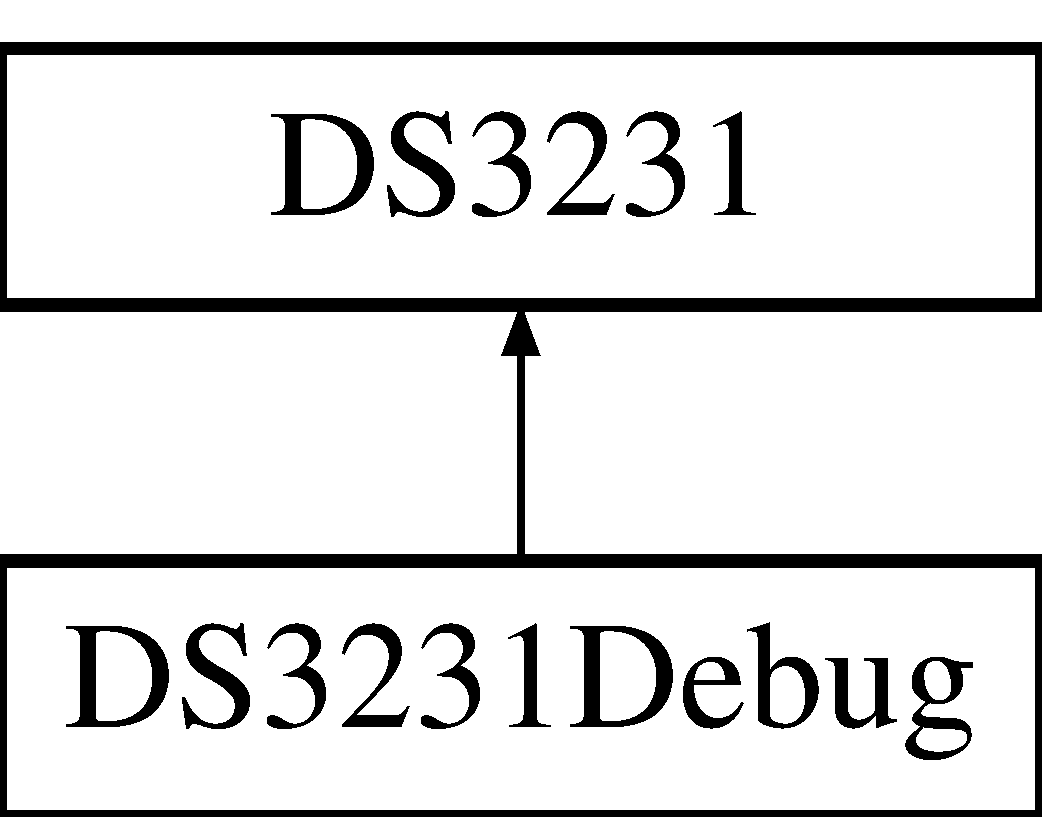
\includegraphics[height=2.000000cm]{class_d_s3231_debug}
\end{center}
\end{figure}
\subsection*{Public Member Functions}
\begin{DoxyCompactItemize}
\item 
virtual void \hyperlink{class_d_s3231_debug_a26f0361e7f1462b1424bb2bb189af240}{dump\+Registers} (Stream $\ast$ser, bool print\+Bitfields=true)
\begin{DoxyCompactList}\small\item\em Dump all registers to serial port. \end{DoxyCompactList}\item 
virtual void \hyperlink{class_d_s3231_debug_a1e95a14a76374cf459d5e4ccbdb6286e}{print\+Register} (Stream $\ast$ser, uint8\+\_\+t reg, bool print\+Bitfields=true)
\begin{DoxyCompactList}\small\item\em Print register and value. \end{DoxyCompactList}\item 
virtual void \hyperlink{class_d_s3231_debug_ac739b6f1980b8254e57b6966ab1dcc97}{print\+Register\+Bitfields} (Stream $\ast$ser, uint8\+\_\+t reg, uint8\+\_\+t reg\+Val)
\begin{DoxyCompactList}\small\item\em Print register bitfields. \end{DoxyCompactList}\item 
virtual void \hyperlink{class_d_s3231_debug_ae9b7944902fc05ea5dcb608c75564f6a}{print\+Diagnostics} (Stream $\ast$ser)
\begin{DoxyCompactList}\small\item\em Print diagnostics. \end{DoxyCompactList}\end{DoxyCompactItemize}


\subsection{Detailed Description}
\hyperlink{class_d_s3231}{D\+S3231} R\+TC debug class. 

The output will be redirected to a user defined serial port. This class can be used by advanced developers to print internal R\+TC registers and diagnostics. Keep in mind that all strings used in this class are flash consuming. 

Definition at line 48 of file Erriez\+D\+S3231\+\_\+debug.\+h.



\subsection{Member Function Documentation}
\index{D\+S3231\+Debug@{D\+S3231\+Debug}!dump\+Registers@{dump\+Registers}}
\index{dump\+Registers@{dump\+Registers}!D\+S3231\+Debug@{D\+S3231\+Debug}}
\subsubsection[{\texorpdfstring{dump\+Registers(\+Stream $\ast$ser, bool print\+Bitfields=true)}{dumpRegisters(Stream *ser, bool printBitfields=true)}}]{\setlength{\rightskip}{0pt plus 5cm}void D\+S3231\+Debug\+::dump\+Registers (
\begin{DoxyParamCaption}
\item[{Stream $\ast$}]{ser, }
\item[{bool}]{print\+Bitfields = {\ttfamily true}}
\end{DoxyParamCaption}
)\hspace{0.3cm}{\ttfamily [virtual]}}\hypertarget{class_d_s3231_debug_a26f0361e7f1462b1424bb2bb189af240}{}\label{class_d_s3231_debug_a26f0361e7f1462b1424bb2bb189af240}


Dump all registers to serial port. 


\begin{DoxyParams}{Parameters}
{\em ser} & Serial port. \\
\hline
{\em print\+Bitfields} & true\+: Print register bitfields. \\
\hline
\end{DoxyParams}


Definition at line 76 of file Erriez\+D\+S3231\+\_\+debug.\+cpp.

\index{D\+S3231\+Debug@{D\+S3231\+Debug}!print\+Diagnostics@{print\+Diagnostics}}
\index{print\+Diagnostics@{print\+Diagnostics}!D\+S3231\+Debug@{D\+S3231\+Debug}}
\subsubsection[{\texorpdfstring{print\+Diagnostics(\+Stream $\ast$ser)}{printDiagnostics(Stream *ser)}}]{\setlength{\rightskip}{0pt plus 5cm}void D\+S3231\+Debug\+::print\+Diagnostics (
\begin{DoxyParamCaption}
\item[{Stream $\ast$}]{ser}
\end{DoxyParamCaption}
)\hspace{0.3cm}{\ttfamily [virtual]}}\hypertarget{class_d_s3231_debug_ae9b7944902fc05ea5dcb608c75564f6a}{}\label{class_d_s3231_debug_ae9b7944902fc05ea5dcb608c75564f6a}


Print diagnostics. 


\begin{DoxyParams}{Parameters}
{\em ser} & Serial port. \\
\hline
\end{DoxyParams}


Definition at line 290 of file Erriez\+D\+S3231\+\_\+debug.\+cpp.

\index{D\+S3231\+Debug@{D\+S3231\+Debug}!print\+Register@{print\+Register}}
\index{print\+Register@{print\+Register}!D\+S3231\+Debug@{D\+S3231\+Debug}}
\subsubsection[{\texorpdfstring{print\+Register(\+Stream $\ast$ser, uint8\+\_\+t reg, bool print\+Bitfields=true)}{printRegister(Stream *ser, uint8_t reg, bool printBitfields=true)}}]{\setlength{\rightskip}{0pt plus 5cm}void D\+S3231\+Debug\+::print\+Register (
\begin{DoxyParamCaption}
\item[{Stream $\ast$}]{ser, }
\item[{uint8\+\_\+t}]{reg, }
\item[{bool}]{print\+Bitfields = {\ttfamily true}}
\end{DoxyParamCaption}
)\hspace{0.3cm}{\ttfamily [virtual]}}\hypertarget{class_d_s3231_debug_a1e95a14a76374cf459d5e4ccbdb6286e}{}\label{class_d_s3231_debug_a1e95a14a76374cf459d5e4ccbdb6286e}


Print register and value. 


\begin{DoxyParams}{Parameters}
{\em ser} & Serial port. \\
\hline
{\em reg} & Register number. \\
\hline
{\em print\+Bitfields} & true\+: Print register bitfields. \\
\hline
\end{DoxyParams}


Definition at line 93 of file Erriez\+D\+S3231\+\_\+debug.\+cpp.

\index{D\+S3231\+Debug@{D\+S3231\+Debug}!print\+Register\+Bitfields@{print\+Register\+Bitfields}}
\index{print\+Register\+Bitfields@{print\+Register\+Bitfields}!D\+S3231\+Debug@{D\+S3231\+Debug}}
\subsubsection[{\texorpdfstring{print\+Register\+Bitfields(\+Stream $\ast$ser, uint8\+\_\+t reg, uint8\+\_\+t reg\+Val)}{printRegisterBitfields(Stream *ser, uint8_t reg, uint8_t regVal)}}]{\setlength{\rightskip}{0pt plus 5cm}void D\+S3231\+Debug\+::print\+Register\+Bitfields (
\begin{DoxyParamCaption}
\item[{Stream $\ast$}]{ser, }
\item[{uint8\+\_\+t}]{reg, }
\item[{uint8\+\_\+t}]{reg\+Val}
\end{DoxyParamCaption}
)\hspace{0.3cm}{\ttfamily [virtual]}}\hypertarget{class_d_s3231_debug_ac739b6f1980b8254e57b6966ab1dcc97}{}\label{class_d_s3231_debug_ac739b6f1980b8254e57b6966ab1dcc97}


Print register bitfields. 


\begin{DoxyParams}{Parameters}
{\em ser} & Serial port. \\
\hline
{\em reg} & Register number. \\
\hline
{\em reg\+Val} & Register value. \\
\hline
\end{DoxyParams}


Definition at line 120 of file Erriez\+D\+S3231\+\_\+debug.\+cpp.



The documentation for this class was generated from the following files\+:\begin{DoxyCompactItemize}
\item 
\hyperlink{_erriez_d_s3231__debug_8h}{Erriez\+D\+S3231\+\_\+debug.\+h}\item 
\hyperlink{_erriez_d_s3231__debug_8cpp}{Erriez\+D\+S3231\+\_\+debug.\+cpp}\end{DoxyCompactItemize}

\chapter{File Documentation}
\hypertarget{_erriez_d_s3231_8cpp}{}\section{Erriez\+D\+S3231.\+cpp File Reference}
\label{_erriez_d_s3231_8cpp}\index{Erriez\+D\+S3231.\+cpp@{Erriez\+D\+S3231.\+cpp}}


\hyperlink{class_d_s3231}{D\+S3231} high precision R\+TC library for Arduino.  


{\ttfamily \#include $<$pgmspace.\+h$>$}\\*
{\ttfamily \#include $<$Wire.\+h$>$}\\*
{\ttfamily \#include \char`\"{}Erriez\+D\+S3231.\+h\char`\"{}}\\*
\subsection*{Variables}
\begin{DoxyCompactItemize}
\item 
const uint8\+\_\+t days\+Month\mbox{[}12\mbox{]} \hyperlink{_erriez_d_s3231_8cpp_ac1d72923583dac3a4d130d5504fd199e}{P\+R\+O\+G\+M\+EM} = \{31, 28, 31, 30, 31, 30, 31, 31, 30, 31, 30, 31\}\hypertarget{_erriez_d_s3231_8cpp_ac1d72923583dac3a4d130d5504fd199e}{}\label{_erriez_d_s3231_8cpp_ac1d72923583dac3a4d130d5504fd199e}

\begin{DoxyCompactList}\small\item\em Define number of days in a month once in flash. \end{DoxyCompactList}\end{DoxyCompactItemize}


\subsection{Detailed Description}
\hyperlink{class_d_s3231}{D\+S3231} high precision R\+TC library for Arduino. 

Source\+: \href{https://github.com/Erriez/ErriezDS3231}{\tt https\+://github.\+com/\+Erriez/\+Erriez\+D\+S3231} Documentation\+: \href{https://erriez.github.io/ErriezDS3231}{\tt https\+://erriez.\+github.\+io/\+Erriez\+D\+S3231} 
\hypertarget{_erriez_d_s3231_8h}{}\section{Erriez\+D\+S3231.\+h File Reference}
\label{_erriez_d_s3231_8h}\index{Erriez\+D\+S3231.\+h@{Erriez\+D\+S3231.\+h}}


\hyperlink{class_d_s3231}{D\+S3231} high precision R\+TC library for Arduino.  


{\ttfamily \#include $<$stdint.\+h$>$}\\*
\subsection*{Classes}
\begin{DoxyCompactItemize}
\item 
struct \hyperlink{struct_d_s3231___date_time__s}{D\+S3231\+\_\+\+Date\+Time\+\_\+s}
\begin{DoxyCompactList}\small\item\em Date time structure. \end{DoxyCompactList}\item 
class \hyperlink{class_d_s3231}{D\+S3231}
\begin{DoxyCompactList}\small\item\em \hyperlink{class_d_s3231}{D\+S3231} R\+TC base class. \end{DoxyCompactList}\end{DoxyCompactItemize}
\subsection*{Macros}
\begin{DoxyCompactItemize}
\item 
\#define \hyperlink{_erriez_d_s3231_8h_ab752aeeb9f43f088ef3ea1e92cf0dd55}{D\+S3231\+\_\+\+R\+E\+G\+\_\+\+S\+E\+C\+O\+N\+DS}~0x00
\begin{DoxyCompactList}\small\item\em \hyperlink{class_d_s3231}{D\+S3231} registers. \end{DoxyCompactList}\item 
\#define \hyperlink{_erriez_d_s3231_8h_a0beecd98fb52521b3df1fb020e10bde1}{D\+S3231\+\_\+\+R\+E\+G\+\_\+\+M\+I\+N\+U\+T\+ES}~0x01\hypertarget{_erriez_d_s3231_8h_a0beecd98fb52521b3df1fb020e10bde1}{}\label{_erriez_d_s3231_8h_a0beecd98fb52521b3df1fb020e10bde1}

\begin{DoxyCompactList}\small\item\em Minutes register. \end{DoxyCompactList}\item 
\#define \hyperlink{_erriez_d_s3231_8h_ac54475e0a15745f77a8275a4ddd71574}{D\+S3231\+\_\+\+R\+E\+G\+\_\+\+H\+O\+U\+RS}~0x02\hypertarget{_erriez_d_s3231_8h_ac54475e0a15745f77a8275a4ddd71574}{}\label{_erriez_d_s3231_8h_ac54475e0a15745f77a8275a4ddd71574}

\begin{DoxyCompactList}\small\item\em Hours register. \end{DoxyCompactList}\item 
\#define \hyperlink{_erriez_d_s3231_8h_a16137f72b183abde987bc1955e9a79ec}{D\+S3231\+\_\+\+R\+E\+G\+\_\+\+D\+A\+Y\+\_\+\+W\+E\+EK}~0x03\hypertarget{_erriez_d_s3231_8h_a16137f72b183abde987bc1955e9a79ec}{}\label{_erriez_d_s3231_8h_a16137f72b183abde987bc1955e9a79ec}

\begin{DoxyCompactList}\small\item\em Day of the week register. \end{DoxyCompactList}\item 
\#define \hyperlink{_erriez_d_s3231_8h_a38ba43f167d51cb2ddd6a9a0b0474a63}{D\+S3231\+\_\+\+R\+E\+G\+\_\+\+D\+A\+Y\+\_\+\+M\+O\+N\+TH}~0x04\hypertarget{_erriez_d_s3231_8h_a38ba43f167d51cb2ddd6a9a0b0474a63}{}\label{_erriez_d_s3231_8h_a38ba43f167d51cb2ddd6a9a0b0474a63}

\begin{DoxyCompactList}\small\item\em Day of the month register. \end{DoxyCompactList}\item 
\#define \hyperlink{_erriez_d_s3231_8h_aaa4a129d3a1b54e2ab4e77f43a6f4985}{D\+S3231\+\_\+\+R\+E\+G\+\_\+\+M\+O\+N\+TH}~0x05\hypertarget{_erriez_d_s3231_8h_aaa4a129d3a1b54e2ab4e77f43a6f4985}{}\label{_erriez_d_s3231_8h_aaa4a129d3a1b54e2ab4e77f43a6f4985}

\begin{DoxyCompactList}\small\item\em Month register. \end{DoxyCompactList}\item 
\#define \hyperlink{_erriez_d_s3231_8h_a109bb0d6f731ff9453434eb80ded18b3}{D\+S3231\+\_\+\+R\+E\+G\+\_\+\+Y\+E\+AR}~0x06\hypertarget{_erriez_d_s3231_8h_a109bb0d6f731ff9453434eb80ded18b3}{}\label{_erriez_d_s3231_8h_a109bb0d6f731ff9453434eb80ded18b3}

\begin{DoxyCompactList}\small\item\em Year register. \end{DoxyCompactList}\item 
\#define \hyperlink{_erriez_d_s3231_8h_afede8b4cdb06307b94e39f7e7022e4c7}{D\+S3231\+\_\+\+R\+E\+G\+\_\+\+A\+L\+A\+R\+M1\+\_\+\+S\+EC}~0x07\hypertarget{_erriez_d_s3231_8h_afede8b4cdb06307b94e39f7e7022e4c7}{}\label{_erriez_d_s3231_8h_afede8b4cdb06307b94e39f7e7022e4c7}

\begin{DoxyCompactList}\small\item\em Alarm 1 seconds register. \end{DoxyCompactList}\item 
\#define \hyperlink{_erriez_d_s3231_8h_ad7f83912c77ff5374d47edd2e3b9843e}{D\+S3231\+\_\+\+R\+E\+G\+\_\+\+A\+L\+A\+R\+M1\+\_\+\+M\+IN}~0x08\hypertarget{_erriez_d_s3231_8h_ad7f83912c77ff5374d47edd2e3b9843e}{}\label{_erriez_d_s3231_8h_ad7f83912c77ff5374d47edd2e3b9843e}

\begin{DoxyCompactList}\small\item\em Alarm 1 minutes register. \end{DoxyCompactList}\item 
\#define \hyperlink{_erriez_d_s3231_8h_ab30cb34cc65cc911e01ed418cf273d54}{D\+S3231\+\_\+\+R\+E\+G\+\_\+\+A\+L\+A\+R\+M1\+\_\+\+H\+O\+UR}~0x09\hypertarget{_erriez_d_s3231_8h_ab30cb34cc65cc911e01ed418cf273d54}{}\label{_erriez_d_s3231_8h_ab30cb34cc65cc911e01ed418cf273d54}

\begin{DoxyCompactList}\small\item\em Alarm 1 hour register. \end{DoxyCompactList}\item 
\#define \hyperlink{_erriez_d_s3231_8h_a77415eaa4adcef6c6c4ee273e662d241}{D\+S3231\+\_\+\+R\+E\+G\+\_\+\+A\+L\+A\+R\+M1\+\_\+\+DD}~0x0A\hypertarget{_erriez_d_s3231_8h_a77415eaa4adcef6c6c4ee273e662d241}{}\label{_erriez_d_s3231_8h_a77415eaa4adcef6c6c4ee273e662d241}

\begin{DoxyCompactList}\small\item\em Alarm 1 day/date register. \end{DoxyCompactList}\item 
\#define \hyperlink{_erriez_d_s3231_8h_a5abe62488283b5ff19c37a32c8fec960}{D\+S3231\+\_\+\+R\+E\+G\+\_\+\+A\+L\+A\+R\+M2\+\_\+\+M\+IN}~0x0B\hypertarget{_erriez_d_s3231_8h_a5abe62488283b5ff19c37a32c8fec960}{}\label{_erriez_d_s3231_8h_a5abe62488283b5ff19c37a32c8fec960}

\begin{DoxyCompactList}\small\item\em Alarm 2 seconds register. \end{DoxyCompactList}\item 
\#define \hyperlink{_erriez_d_s3231_8h_a8f1242d9ac14bd6587ff421612d71d5d}{D\+S3231\+\_\+\+R\+E\+G\+\_\+\+A\+L\+A\+R\+M2\+\_\+\+H\+O\+UR}~0x0C\hypertarget{_erriez_d_s3231_8h_a8f1242d9ac14bd6587ff421612d71d5d}{}\label{_erriez_d_s3231_8h_a8f1242d9ac14bd6587ff421612d71d5d}

\begin{DoxyCompactList}\small\item\em Alarm 2 hour register. \end{DoxyCompactList}\item 
\#define \hyperlink{_erriez_d_s3231_8h_a0d3aef73a55babba7ce7d5e17447f8fa}{D\+S3231\+\_\+\+R\+E\+G\+\_\+\+A\+L\+A\+R\+M2\+\_\+\+DD}~0x0D\hypertarget{_erriez_d_s3231_8h_a0d3aef73a55babba7ce7d5e17447f8fa}{}\label{_erriez_d_s3231_8h_a0d3aef73a55babba7ce7d5e17447f8fa}

\begin{DoxyCompactList}\small\item\em Alarm 2 day/date register. \end{DoxyCompactList}\item 
\#define \hyperlink{_erriez_d_s3231_8h_a14b27d8bc32c34f1eaecf569355c84d3}{D\+S3231\+\_\+\+R\+E\+G\+\_\+\+C\+O\+N\+T\+R\+OL}~0x0E\hypertarget{_erriez_d_s3231_8h_a14b27d8bc32c34f1eaecf569355c84d3}{}\label{_erriez_d_s3231_8h_a14b27d8bc32c34f1eaecf569355c84d3}

\begin{DoxyCompactList}\small\item\em Control register. \end{DoxyCompactList}\item 
\#define \hyperlink{_erriez_d_s3231_8h_aeee46891f279544efa92a99e15e8d023}{D\+S3231\+\_\+\+R\+E\+G\+\_\+\+S\+T\+A\+T\+US}~0x0F\hypertarget{_erriez_d_s3231_8h_aeee46891f279544efa92a99e15e8d023}{}\label{_erriez_d_s3231_8h_aeee46891f279544efa92a99e15e8d023}

\begin{DoxyCompactList}\small\item\em Status register. \end{DoxyCompactList}\item 
\#define \hyperlink{_erriez_d_s3231_8h_a2c630e7f3a057480946da744449d2eb3}{D\+S3231\+\_\+\+R\+E\+G\+\_\+\+A\+G\+I\+N\+G\+\_\+\+O\+F\+F\+S\+ET}~0x10\hypertarget{_erriez_d_s3231_8h_a2c630e7f3a057480946da744449d2eb3}{}\label{_erriez_d_s3231_8h_a2c630e7f3a057480946da744449d2eb3}

\begin{DoxyCompactList}\small\item\em Aging offset register. \end{DoxyCompactList}\item 
\#define \hyperlink{_erriez_d_s3231_8h_aa03c8831a5b1e11abc00e730c23ecc55}{D\+S3231\+\_\+\+R\+E\+G\+\_\+\+T\+E\+M\+P\+\_\+\+M\+SB}~0x11\hypertarget{_erriez_d_s3231_8h_aa03c8831a5b1e11abc00e730c23ecc55}{}\label{_erriez_d_s3231_8h_aa03c8831a5b1e11abc00e730c23ecc55}

\begin{DoxyCompactList}\small\item\em Temperature M\+SB register. \end{DoxyCompactList}\item 
\#define \hyperlink{_erriez_d_s3231_8h_a35ddcaf5258fc941f90f8428c2032fa1}{D\+S3231\+\_\+\+R\+E\+G\+\_\+\+T\+E\+M\+P\+\_\+\+L\+SB}~0x12\hypertarget{_erriez_d_s3231_8h_a35ddcaf5258fc941f90f8428c2032fa1}{}\label{_erriez_d_s3231_8h_a35ddcaf5258fc941f90f8428c2032fa1}

\begin{DoxyCompactList}\small\item\em Temperature L\+SB register. \end{DoxyCompactList}\item 
\#define \hyperlink{_erriez_d_s3231_8h_aa2b7ed3fc2a05cd3492ded65a51c4bcd}{D\+S3231\+\_\+\+N\+U\+M\+\_\+\+R\+E\+GS}~19
\begin{DoxyCompactList}\small\item\em \hyperlink{class_d_s3231}{D\+S3231} number of registers. \end{DoxyCompactList}\item 
\#define \hyperlink{_erriez_d_s3231_8h_afc86f3d550d154199d3e529597b8a183}{D\+S3231\+\_\+\+H\+O\+U\+R\+\_\+12\+H\+\_\+24H}~6
\begin{DoxyCompactList}\small\item\em \hyperlink{class_d_s3231}{D\+S3231} register bit defines. \end{DoxyCompactList}\item 
\#define \hyperlink{_erriez_d_s3231_8h_ac6f6f14cb51361e5f43e23943452dd7c}{D\+S3231\+\_\+\+H\+O\+U\+R\+\_\+\+A\+M\+\_\+\+PM}~5\hypertarget{_erriez_d_s3231_8h_ac6f6f14cb51361e5f43e23943452dd7c}{}\label{_erriez_d_s3231_8h_ac6f6f14cb51361e5f43e23943452dd7c}

\begin{DoxyCompactList}\small\item\em A\+M/\+PM. \end{DoxyCompactList}\item 
\#define \hyperlink{_erriez_d_s3231_8h_a36a2f718d3519e257c563725a3e995b3}{D\+S3231\+\_\+\+M\+O\+N\+T\+H\+\_\+\+C\+E\+N\+T\+U\+RY}~7\hypertarget{_erriez_d_s3231_8h_a36a2f718d3519e257c563725a3e995b3}{}\label{_erriez_d_s3231_8h_a36a2f718d3519e257c563725a3e995b3}

\begin{DoxyCompactList}\small\item\em Century. \end{DoxyCompactList}\item 
\#define \hyperlink{_erriez_d_s3231_8h_acfc1677178811d53cd457c4880c54ccc}{D\+S3231\+\_\+\+C\+T\+R\+L\+\_\+\+E\+O\+SC}~7\hypertarget{_erriez_d_s3231_8h_acfc1677178811d53cd457c4880c54ccc}{}\label{_erriez_d_s3231_8h_acfc1677178811d53cd457c4880c54ccc}

\begin{DoxyCompactList}\small\item\em Enable oscillator. \end{DoxyCompactList}\item 
\#define \hyperlink{_erriez_d_s3231_8h_ae1cc580bf1a5bfb3986e4d779ac6b038}{D\+S3231\+\_\+\+C\+T\+R\+L\+\_\+\+B\+B\+S\+QW}~6\hypertarget{_erriez_d_s3231_8h_ae1cc580bf1a5bfb3986e4d779ac6b038}{}\label{_erriez_d_s3231_8h_ae1cc580bf1a5bfb3986e4d779ac6b038}

\begin{DoxyCompactList}\small\item\em Battery-\/\+Backed Square-\/\+Wave Enable. \end{DoxyCompactList}\item 
\#define \hyperlink{_erriez_d_s3231_8h_a85eb927c3762783eed85ceebb1c043ab}{D\+S3231\+\_\+\+C\+T\+R\+L\+\_\+\+C\+O\+NV}~5\hypertarget{_erriez_d_s3231_8h_a85eb927c3762783eed85ceebb1c043ab}{}\label{_erriez_d_s3231_8h_a85eb927c3762783eed85ceebb1c043ab}

\begin{DoxyCompactList}\small\item\em Start temperature conversion. \end{DoxyCompactList}\item 
\#define \hyperlink{_erriez_d_s3231_8h_ad6d9343d99d0781547085e4738550a9b}{D\+S3231\+\_\+\+C\+T\+R\+L\+\_\+\+R\+S2}~4\hypertarget{_erriez_d_s3231_8h_ad6d9343d99d0781547085e4738550a9b}{}\label{_erriez_d_s3231_8h_ad6d9343d99d0781547085e4738550a9b}

\begin{DoxyCompactList}\small\item\em Square wave rate-\/select 2. \end{DoxyCompactList}\item 
\#define \hyperlink{_erriez_d_s3231_8h_a73c83c329cb1cb19a4d3041f5c96efb7}{D\+S3231\+\_\+\+C\+T\+R\+L\+\_\+\+R\+S1}~3\hypertarget{_erriez_d_s3231_8h_a73c83c329cb1cb19a4d3041f5c96efb7}{}\label{_erriez_d_s3231_8h_a73c83c329cb1cb19a4d3041f5c96efb7}

\begin{DoxyCompactList}\small\item\em Square wave rate-\/select 1. \end{DoxyCompactList}\item 
\#define \hyperlink{_erriez_d_s3231_8h_a52c8ae1dab4ea9e3228283fbd7067429}{D\+S3231\+\_\+\+C\+T\+R\+L\+\_\+\+I\+N\+T\+CN}~2\hypertarget{_erriez_d_s3231_8h_a52c8ae1dab4ea9e3228283fbd7067429}{}\label{_erriez_d_s3231_8h_a52c8ae1dab4ea9e3228283fbd7067429}

\begin{DoxyCompactList}\small\item\em Interrupt control. \end{DoxyCompactList}\item 
\#define \hyperlink{_erriez_d_s3231_8h_af410370b8fe4ae2230aff4f9677c80ef}{D\+S3231\+\_\+\+C\+T\+R\+L\+\_\+\+A2\+IE}~1\hypertarget{_erriez_d_s3231_8h_af410370b8fe4ae2230aff4f9677c80ef}{}\label{_erriez_d_s3231_8h_af410370b8fe4ae2230aff4f9677c80ef}

\begin{DoxyCompactList}\small\item\em Alarm 2 interrupt enable. \end{DoxyCompactList}\item 
\#define \hyperlink{_erriez_d_s3231_8h_acba36e31094c1ca15def397a8b3fa6c7}{D\+S3231\+\_\+\+C\+T\+R\+L\+\_\+\+A1\+IE}~0\hypertarget{_erriez_d_s3231_8h_acba36e31094c1ca15def397a8b3fa6c7}{}\label{_erriez_d_s3231_8h_acba36e31094c1ca15def397a8b3fa6c7}

\begin{DoxyCompactList}\small\item\em Alarm 1 interrupt enable. \end{DoxyCompactList}\item 
\#define \hyperlink{_erriez_d_s3231_8h_a5c397f0a0fc1b58781ae42769c0e3acb}{D\+S3231\+\_\+\+S\+T\+A\+T\+\_\+\+O\+SF}~7\hypertarget{_erriez_d_s3231_8h_a5c397f0a0fc1b58781ae42769c0e3acb}{}\label{_erriez_d_s3231_8h_a5c397f0a0fc1b58781ae42769c0e3acb}

\begin{DoxyCompactList}\small\item\em Oscillator Stop Flag. \end{DoxyCompactList}\item 
\#define \hyperlink{_erriez_d_s3231_8h_ab9c9d4f03dde9fbd46f9622057374290}{D\+S3231\+\_\+\+S\+T\+A\+T\+\_\+\+E\+N32\+K\+HZ}~3\hypertarget{_erriez_d_s3231_8h_ab9c9d4f03dde9fbd46f9622057374290}{}\label{_erriez_d_s3231_8h_ab9c9d4f03dde9fbd46f9622057374290}

\begin{DoxyCompactList}\small\item\em Enable 32k\+Hz clock output. \end{DoxyCompactList}\item 
\#define \hyperlink{_erriez_d_s3231_8h_ad8803f7c4831af86871021f0d19dacd8}{D\+S3231\+\_\+\+S\+T\+A\+T\+\_\+\+B\+SY}~2\hypertarget{_erriez_d_s3231_8h_ad8803f7c4831af86871021f0d19dacd8}{}\label{_erriez_d_s3231_8h_ad8803f7c4831af86871021f0d19dacd8}

\begin{DoxyCompactList}\small\item\em Temperature conversion busy flag. \end{DoxyCompactList}\item 
\#define \hyperlink{_erriez_d_s3231_8h_a7be6975286363e086069e64c1e8508d7}{D\+S3231\+\_\+\+S\+T\+A\+T\+\_\+\+A2F}~1\hypertarget{_erriez_d_s3231_8h_a7be6975286363e086069e64c1e8508d7}{}\label{_erriez_d_s3231_8h_a7be6975286363e086069e64c1e8508d7}

\begin{DoxyCompactList}\small\item\em Alarm 2 status flag. \end{DoxyCompactList}\item 
\#define \hyperlink{_erriez_d_s3231_8h_ad22da5484f82ad0ad700cca4987f31bd}{D\+S3231\+\_\+\+S\+T\+A\+T\+\_\+\+A1F}~0\hypertarget{_erriez_d_s3231_8h_ad22da5484f82ad0ad700cca4987f31bd}{}\label{_erriez_d_s3231_8h_ad22da5484f82ad0ad700cca4987f31bd}

\begin{DoxyCompactList}\small\item\em Alarm 1 status flag. \end{DoxyCompactList}\item 
\#define \hyperlink{_erriez_d_s3231_8h_a8c1ec90975663dd3fbf3af437e3746f2}{D\+S3231\+\_\+\+A1\+M1}~7\hypertarget{_erriez_d_s3231_8h_a8c1ec90975663dd3fbf3af437e3746f2}{}\label{_erriez_d_s3231_8h_a8c1ec90975663dd3fbf3af437e3746f2}

\begin{DoxyCompactList}\small\item\em Alarm 1 bit 7 seconds register. \end{DoxyCompactList}\item 
\#define \hyperlink{_erriez_d_s3231_8h_a26ad907956857109f1e7541534346b35}{D\+S3231\+\_\+\+A1\+M2}~7\hypertarget{_erriez_d_s3231_8h_a26ad907956857109f1e7541534346b35}{}\label{_erriez_d_s3231_8h_a26ad907956857109f1e7541534346b35}

\begin{DoxyCompactList}\small\item\em Alarm 1 bit 7 minutes register. \end{DoxyCompactList}\item 
\#define \hyperlink{_erriez_d_s3231_8h_a394d188c724a278704fceca92985d01d}{D\+S3231\+\_\+\+A1\+M3}~7\hypertarget{_erriez_d_s3231_8h_a394d188c724a278704fceca92985d01d}{}\label{_erriez_d_s3231_8h_a394d188c724a278704fceca92985d01d}

\begin{DoxyCompactList}\small\item\em Alarm 1 bit 7 hours register. \end{DoxyCompactList}\item 
\#define \hyperlink{_erriez_d_s3231_8h_a8e281311ab191af539eeb25c8044d834}{D\+S3231\+\_\+\+A1\+M4}~7\hypertarget{_erriez_d_s3231_8h_a8e281311ab191af539eeb25c8044d834}{}\label{_erriez_d_s3231_8h_a8e281311ab191af539eeb25c8044d834}

\begin{DoxyCompactList}\small\item\em Alarm 1 bit 7 day/date register. \end{DoxyCompactList}\item 
\#define \hyperlink{_erriez_d_s3231_8h_a5a5aff588c7b314b0f5bfbfaad4e2757}{D\+S3231\+\_\+\+A2\+M2}~7\hypertarget{_erriez_d_s3231_8h_a5a5aff588c7b314b0f5bfbfaad4e2757}{}\label{_erriez_d_s3231_8h_a5a5aff588c7b314b0f5bfbfaad4e2757}

\begin{DoxyCompactList}\small\item\em Alarm 2 bit 7 minutes register. \end{DoxyCompactList}\item 
\#define \hyperlink{_erriez_d_s3231_8h_af3283fe891bcf24f833632b5457ade22}{D\+S3231\+\_\+\+A2\+M3}~7\hypertarget{_erriez_d_s3231_8h_af3283fe891bcf24f833632b5457ade22}{}\label{_erriez_d_s3231_8h_af3283fe891bcf24f833632b5457ade22}

\begin{DoxyCompactList}\small\item\em Alarm 2 bit 7 hours register. \end{DoxyCompactList}\item 
\#define \hyperlink{_erriez_d_s3231_8h_a0998f99cb5e5e92560d0aa18cc8016c8}{D\+S3231\+\_\+\+A2\+M4}~7\hypertarget{_erriez_d_s3231_8h_a0998f99cb5e5e92560d0aa18cc8016c8}{}\label{_erriez_d_s3231_8h_a0998f99cb5e5e92560d0aa18cc8016c8}

\begin{DoxyCompactList}\small\item\em Alarm 2 bit 7 day/date register. \end{DoxyCompactList}\item 
\#define \hyperlink{_erriez_d_s3231_8h_a038d89a9fa0ed2aa02a023cb67416116}{D\+S3231\+\_\+\+D\+Y\+DT}~6\hypertarget{_erriez_d_s3231_8h_a038d89a9fa0ed2aa02a023cb67416116}{}\label{_erriez_d_s3231_8h_a038d89a9fa0ed2aa02a023cb67416116}

\begin{DoxyCompactList}\small\item\em Alarm 2 bit 6. \end{DoxyCompactList}\item 
\#define \hyperlink{_erriez_d_s3231_8h_a807ca712a5ee10a56cf420c420c42524}{D\+S3231\+\_\+\+A\+D\+DR}~(0x\+D0 $>$$>$ 1)\hypertarget{_erriez_d_s3231_8h_a807ca712a5ee10a56cf420c420c42524}{}\label{_erriez_d_s3231_8h_a807ca712a5ee10a56cf420c420c42524}

\begin{DoxyCompactList}\small\item\em \hyperlink{class_d_s3231}{D\+S3231} I2C 7-\/bit address. \end{DoxyCompactList}\item 
\#define \hyperlink{_erriez_d_s3231_8h_a1a4c3c6b78fa47471646f18b572ddd46}{S\+E\+C\+O\+N\+D\+S\+\_\+\+F\+R\+O\+M\+\_\+1970\+\_\+\+T\+O\+\_\+2000}~946684800\hypertarget{_erriez_d_s3231_8h_a1a4c3c6b78fa47471646f18b572ddd46}{}\label{_erriez_d_s3231_8h_a1a4c3c6b78fa47471646f18b572ddd46}

\begin{DoxyCompactList}\small\item\em Number of seconds between year 1970 and 2000. \end{DoxyCompactList}\end{DoxyCompactItemize}
\subsection*{Typedefs}
\begin{DoxyCompactItemize}
\item 
typedef struct \hyperlink{struct_d_s3231___date_time__s}{D\+S3231\+\_\+\+Date\+Time\+\_\+s} \hyperlink{_erriez_d_s3231_8h_a79a5c1f4b249b6f512ca108013374536}{D\+S3231\+\_\+\+Date\+Time}\hypertarget{_erriez_d_s3231_8h_a79a5c1f4b249b6f512ca108013374536}{}\label{_erriez_d_s3231_8h_a79a5c1f4b249b6f512ca108013374536}

\begin{DoxyCompactList}\small\item\em Date time structure. \end{DoxyCompactList}\end{DoxyCompactItemize}
\subsection*{Enumerations}
\begin{DoxyCompactItemize}
\item 
enum \hyperlink{_erriez_d_s3231_8h_abdac868b647b120d540abd60d35e0feb}{Alarm\+Id} \{ \hyperlink{_erriez_d_s3231_8h_abdac868b647b120d540abd60d35e0feba570a34fc2ad752afdd9d32adebe1bcf0}{Alarm1} = 1, 
\hyperlink{_erriez_d_s3231_8h_abdac868b647b120d540abd60d35e0feba1cbf027c32d10b347dd30cfbfb2b4c2a}{Alarm2} = 2
 \}\begin{DoxyCompactList}\small\item\em Alarm ID. \end{DoxyCompactList}
\item 
enum \hyperlink{_erriez_d_s3231_8h_aa29471da8f6d22930cc9159a55a49273}{Alarm1\+Type} \{ \\*
\hyperlink{_erriez_d_s3231_8h_aa29471da8f6d22930cc9159a55a49273a9ad7fb7e52143b498c8719cd55ea0e75}{Alarm1\+Every\+Second} = 0x0F, 
\hyperlink{_erriez_d_s3231_8h_aa29471da8f6d22930cc9159a55a49273a0591ae10bff7a049677ee1b51a92cef0}{Alarm1\+Match\+Seconds} = 0x0E, 
\hyperlink{_erriez_d_s3231_8h_aa29471da8f6d22930cc9159a55a49273a507714a41f83ccaaecd07d3a3826bba7}{Alarm1\+Match\+Minutes} = 0x0C, 
\hyperlink{_erriez_d_s3231_8h_aa29471da8f6d22930cc9159a55a49273af4b6860f0512c98ef636bd0ef501aad6}{Alarm1\+Match\+Hours} = 0x08, 
\\*
\hyperlink{_erriez_d_s3231_8h_aa29471da8f6d22930cc9159a55a49273a0ebac0e1cb2344a20b6003362da04d46}{Alarm1\+Match\+Day} = 0x10, 
\hyperlink{_erriez_d_s3231_8h_aa29471da8f6d22930cc9159a55a49273a81f553292256cec98d307fa1164f6213}{Alarm1\+Match\+Date} = 0x00
 \}\begin{DoxyCompactList}\small\item\em Alarm 1 types enum. \end{DoxyCompactList}
\item 
enum \hyperlink{_erriez_d_s3231_8h_a2561c628950a85b8f502b7055c3acd8b}{Alarm2\+Type} \{ \\*
\hyperlink{_erriez_d_s3231_8h_a2561c628950a85b8f502b7055c3acd8ba16afbf3a37ee40519360ce240189835a}{Alarm2\+Every\+Minute} = 0x0E, 
\hyperlink{_erriez_d_s3231_8h_a2561c628950a85b8f502b7055c3acd8ba31c3bdaa746d32d314e8039b667443d3}{Alarm2\+Match\+Minutes} = 0x0C, 
\hyperlink{_erriez_d_s3231_8h_a2561c628950a85b8f502b7055c3acd8ba3c7273b5f252692d3d08495ec41b593f}{Alarm2\+Match\+Hours} = 0x08, 
\hyperlink{_erriez_d_s3231_8h_a2561c628950a85b8f502b7055c3acd8bad5051960ee85737d724f7161e2be9efc}{Alarm2\+Match\+Day} = 0x10, 
\\*
\hyperlink{_erriez_d_s3231_8h_a2561c628950a85b8f502b7055c3acd8ba1ac76d9841ac88cb1e44a0981a0d7859}{Alarm2\+Match\+Date} = 0x00
 \}\begin{DoxyCompactList}\small\item\em Alarm 2 types enum. \end{DoxyCompactList}
\item 
enum \hyperlink{_erriez_d_s3231_8h_aa45f48b2c6f58f91a278a1601b211140}{Square\+Wave} \{ \\*
\hyperlink{_erriez_d_s3231_8h_aa45f48b2c6f58f91a278a1601b211140a6c1c124acf12e396561ddad9f20eda8b}{Square\+Wave\+Disable} = (1 $<$$<$ D\+S3231\+\_\+\+C\+T\+R\+L\+\_\+\+I\+N\+T\+CN), 
\hyperlink{_erriez_d_s3231_8h_aa45f48b2c6f58f91a278a1601b211140a60273c5ec4e96c0da9bc1d72e2559174}{Square\+Wave1\+Hz} = ((0 $<$$<$ D\+S3231\+\_\+\+C\+T\+R\+L\+\_\+\+R\+S2) $\vert$ (0 $<$$<$ D\+S3231\+\_\+\+C\+T\+R\+L\+\_\+\+R\+S1)), 
\hyperlink{_erriez_d_s3231_8h_aa45f48b2c6f58f91a278a1601b211140abc8fb24c81b6abcc74985aaac7d4ffd9}{Square\+Wave1024\+Hz} = ((0 $<$$<$ D\+S3231\+\_\+\+C\+T\+R\+L\+\_\+\+R\+S2) $\vert$ (1 $<$$<$ D\+S3231\+\_\+\+C\+T\+R\+L\+\_\+\+R\+S1)), 
\hyperlink{_erriez_d_s3231_8h_aa45f48b2c6f58f91a278a1601b211140a69c7b381b660ea601d14f105129b61a9}{Square\+Wave4096\+Hz} = ((1 $<$$<$ D\+S3231\+\_\+\+C\+T\+R\+L\+\_\+\+R\+S2) $\vert$ (0 $<$$<$ D\+S3231\+\_\+\+C\+T\+R\+L\+\_\+\+R\+S1)), 
\\*
\hyperlink{_erriez_d_s3231_8h_aa45f48b2c6f58f91a278a1601b211140a65eb82be2c7cfcc67481df02893a0b9c}{Square\+Wave8192\+Hz} = ((1 $<$$<$ D\+S3231\+\_\+\+C\+T\+R\+L\+\_\+\+R\+S2) $\vert$ (1 $<$$<$ D\+S3231\+\_\+\+C\+T\+R\+L\+\_\+\+R\+S1))
 \}\begin{DoxyCompactList}\small\item\em Squarewave enum. \end{DoxyCompactList}
\end{DoxyCompactItemize}


\subsection{Detailed Description}
\hyperlink{class_d_s3231}{D\+S3231} high precision R\+TC library for Arduino. 

Source\+: \href{https://github.com/Erriez/ErriezDS3231}{\tt https\+://github.\+com/\+Erriez/\+Erriez\+D\+S3231} Documentation\+: \href{https://erriez.github.io/ErriezDS3231}{\tt https\+://erriez.\+github.\+io/\+Erriez\+D\+S3231} 

\subsection{Macro Definition Documentation}
\index{Erriez\+D\+S3231.\+h@{Erriez\+D\+S3231.\+h}!D\+S3231\+\_\+\+H\+O\+U\+R\+\_\+12\+H\+\_\+24H@{D\+S3231\+\_\+\+H\+O\+U\+R\+\_\+12\+H\+\_\+24H}}
\index{D\+S3231\+\_\+\+H\+O\+U\+R\+\_\+12\+H\+\_\+24H@{D\+S3231\+\_\+\+H\+O\+U\+R\+\_\+12\+H\+\_\+24H}!Erriez\+D\+S3231.\+h@{Erriez\+D\+S3231.\+h}}
\subsubsection[{\texorpdfstring{D\+S3231\+\_\+\+H\+O\+U\+R\+\_\+12\+H\+\_\+24H}{DS3231_HOUR_12H_24H}}]{\setlength{\rightskip}{0pt plus 5cm}\#define D\+S3231\+\_\+\+H\+O\+U\+R\+\_\+12\+H\+\_\+24H~6}\hypertarget{_erriez_d_s3231_8h_afc86f3d550d154199d3e529597b8a183}{}\label{_erriez_d_s3231_8h_afc86f3d550d154199d3e529597b8a183}


\hyperlink{class_d_s3231}{D\+S3231} register bit defines. 

12 or 24 hour mode 

Definition at line 65 of file Erriez\+D\+S3231.\+h.

\index{Erriez\+D\+S3231.\+h@{Erriez\+D\+S3231.\+h}!D\+S3231\+\_\+\+N\+U\+M\+\_\+\+R\+E\+GS@{D\+S3231\+\_\+\+N\+U\+M\+\_\+\+R\+E\+GS}}
\index{D\+S3231\+\_\+\+N\+U\+M\+\_\+\+R\+E\+GS@{D\+S3231\+\_\+\+N\+U\+M\+\_\+\+R\+E\+GS}!Erriez\+D\+S3231.\+h@{Erriez\+D\+S3231.\+h}}
\subsubsection[{\texorpdfstring{D\+S3231\+\_\+\+N\+U\+M\+\_\+\+R\+E\+GS}{DS3231_NUM_REGS}}]{\setlength{\rightskip}{0pt plus 5cm}\#define D\+S3231\+\_\+\+N\+U\+M\+\_\+\+R\+E\+GS~19}\hypertarget{_erriez_d_s3231_8h_aa2b7ed3fc2a05cd3492ded65a51c4bcd}{}\label{_erriez_d_s3231_8h_aa2b7ed3fc2a05cd3492ded65a51c4bcd}


\hyperlink{class_d_s3231}{D\+S3231} number of registers. 

19 R\+TC register\+: 0x00..0x12 

Definition at line 62 of file Erriez\+D\+S3231.\+h.

\index{Erriez\+D\+S3231.\+h@{Erriez\+D\+S3231.\+h}!D\+S3231\+\_\+\+R\+E\+G\+\_\+\+S\+E\+C\+O\+N\+DS@{D\+S3231\+\_\+\+R\+E\+G\+\_\+\+S\+E\+C\+O\+N\+DS}}
\index{D\+S3231\+\_\+\+R\+E\+G\+\_\+\+S\+E\+C\+O\+N\+DS@{D\+S3231\+\_\+\+R\+E\+G\+\_\+\+S\+E\+C\+O\+N\+DS}!Erriez\+D\+S3231.\+h@{Erriez\+D\+S3231.\+h}}
\subsubsection[{\texorpdfstring{D\+S3231\+\_\+\+R\+E\+G\+\_\+\+S\+E\+C\+O\+N\+DS}{DS3231_REG_SECONDS}}]{\setlength{\rightskip}{0pt plus 5cm}\#define D\+S3231\+\_\+\+R\+E\+G\+\_\+\+S\+E\+C\+O\+N\+DS~0x00}\hypertarget{_erriez_d_s3231_8h_ab752aeeb9f43f088ef3ea1e92cf0dd55}{}\label{_erriez_d_s3231_8h_ab752aeeb9f43f088ef3ea1e92cf0dd55}


\hyperlink{class_d_s3231}{D\+S3231} registers. 

Seconds register 

Definition at line 39 of file Erriez\+D\+S3231.\+h.



\subsection{Enumeration Type Documentation}
\index{Erriez\+D\+S3231.\+h@{Erriez\+D\+S3231.\+h}!Alarm1\+Type@{Alarm1\+Type}}
\index{Alarm1\+Type@{Alarm1\+Type}!Erriez\+D\+S3231.\+h@{Erriez\+D\+S3231.\+h}}
\subsubsection[{\texorpdfstring{Alarm1\+Type}{Alarm1Type}}]{\setlength{\rightskip}{0pt plus 5cm}enum {\bf Alarm1\+Type}}\hypertarget{_erriez_d_s3231_8h_aa29471da8f6d22930cc9159a55a49273}{}\label{_erriez_d_s3231_8h_aa29471da8f6d22930cc9159a55a49273}


Alarm 1 types enum. 

\begin{Desc}
\item[Enumerator]\par
\begin{description}
\index{Alarm1\+Every\+Second@{Alarm1\+Every\+Second}!Erriez\+D\+S3231.\+h@{Erriez\+D\+S3231.\+h}}\index{Erriez\+D\+S3231.\+h@{Erriez\+D\+S3231.\+h}!Alarm1\+Every\+Second@{Alarm1\+Every\+Second}}\item[{\em 
Alarm1\+Every\+Second\hypertarget{_erriez_d_s3231_8h_aa29471da8f6d22930cc9159a55a49273a9ad7fb7e52143b498c8719cd55ea0e75}{}\label{_erriez_d_s3231_8h_aa29471da8f6d22930cc9159a55a49273a9ad7fb7e52143b498c8719cd55ea0e75}
}]Alarm once per second. \index{Alarm1\+Match\+Seconds@{Alarm1\+Match\+Seconds}!Erriez\+D\+S3231.\+h@{Erriez\+D\+S3231.\+h}}\index{Erriez\+D\+S3231.\+h@{Erriez\+D\+S3231.\+h}!Alarm1\+Match\+Seconds@{Alarm1\+Match\+Seconds}}\item[{\em 
Alarm1\+Match\+Seconds\hypertarget{_erriez_d_s3231_8h_aa29471da8f6d22930cc9159a55a49273a0591ae10bff7a049677ee1b51a92cef0}{}\label{_erriez_d_s3231_8h_aa29471da8f6d22930cc9159a55a49273a0591ae10bff7a049677ee1b51a92cef0}
}]Alarm when seconds match. \index{Alarm1\+Match\+Minutes@{Alarm1\+Match\+Minutes}!Erriez\+D\+S3231.\+h@{Erriez\+D\+S3231.\+h}}\index{Erriez\+D\+S3231.\+h@{Erriez\+D\+S3231.\+h}!Alarm1\+Match\+Minutes@{Alarm1\+Match\+Minutes}}\item[{\em 
Alarm1\+Match\+Minutes\hypertarget{_erriez_d_s3231_8h_aa29471da8f6d22930cc9159a55a49273a507714a41f83ccaaecd07d3a3826bba7}{}\label{_erriez_d_s3231_8h_aa29471da8f6d22930cc9159a55a49273a507714a41f83ccaaecd07d3a3826bba7}
}]Alarm when minutes and seconds match. \index{Alarm1\+Match\+Hours@{Alarm1\+Match\+Hours}!Erriez\+D\+S3231.\+h@{Erriez\+D\+S3231.\+h}}\index{Erriez\+D\+S3231.\+h@{Erriez\+D\+S3231.\+h}!Alarm1\+Match\+Hours@{Alarm1\+Match\+Hours}}\item[{\em 
Alarm1\+Match\+Hours\hypertarget{_erriez_d_s3231_8h_aa29471da8f6d22930cc9159a55a49273af4b6860f0512c98ef636bd0ef501aad6}{}\label{_erriez_d_s3231_8h_aa29471da8f6d22930cc9159a55a49273af4b6860f0512c98ef636bd0ef501aad6}
}]Alarm when hours, minutes, and seconds match. \index{Alarm1\+Match\+Day@{Alarm1\+Match\+Day}!Erriez\+D\+S3231.\+h@{Erriez\+D\+S3231.\+h}}\index{Erriez\+D\+S3231.\+h@{Erriez\+D\+S3231.\+h}!Alarm1\+Match\+Day@{Alarm1\+Match\+Day}}\item[{\em 
Alarm1\+Match\+Day\hypertarget{_erriez_d_s3231_8h_aa29471da8f6d22930cc9159a55a49273a0ebac0e1cb2344a20b6003362da04d46}{}\label{_erriez_d_s3231_8h_aa29471da8f6d22930cc9159a55a49273a0ebac0e1cb2344a20b6003362da04d46}
}]Alarm when date, hours, minutes, and seconds match. \index{Alarm1\+Match\+Date@{Alarm1\+Match\+Date}!Erriez\+D\+S3231.\+h@{Erriez\+D\+S3231.\+h}}\index{Erriez\+D\+S3231.\+h@{Erriez\+D\+S3231.\+h}!Alarm1\+Match\+Date@{Alarm1\+Match\+Date}}\item[{\em 
Alarm1\+Match\+Date\hypertarget{_erriez_d_s3231_8h_aa29471da8f6d22930cc9159a55a49273a81f553292256cec98d307fa1164f6213}{}\label{_erriez_d_s3231_8h_aa29471da8f6d22930cc9159a55a49273a81f553292256cec98d307fa1164f6213}
}]Alarm when day, hours, minutes, and seconds match. \end{description}
\end{Desc}


Definition at line 124 of file Erriez\+D\+S3231.\+h.

\index{Erriez\+D\+S3231.\+h@{Erriez\+D\+S3231.\+h}!Alarm2\+Type@{Alarm2\+Type}}
\index{Alarm2\+Type@{Alarm2\+Type}!Erriez\+D\+S3231.\+h@{Erriez\+D\+S3231.\+h}}
\subsubsection[{\texorpdfstring{Alarm2\+Type}{Alarm2Type}}]{\setlength{\rightskip}{0pt plus 5cm}enum {\bf Alarm2\+Type}}\hypertarget{_erriez_d_s3231_8h_a2561c628950a85b8f502b7055c3acd8b}{}\label{_erriez_d_s3231_8h_a2561c628950a85b8f502b7055c3acd8b}


Alarm 2 types enum. 

\begin{Desc}
\item[Enumerator]\par
\begin{description}
\index{Alarm2\+Every\+Minute@{Alarm2\+Every\+Minute}!Erriez\+D\+S3231.\+h@{Erriez\+D\+S3231.\+h}}\index{Erriez\+D\+S3231.\+h@{Erriez\+D\+S3231.\+h}!Alarm2\+Every\+Minute@{Alarm2\+Every\+Minute}}\item[{\em 
Alarm2\+Every\+Minute\hypertarget{_erriez_d_s3231_8h_a2561c628950a85b8f502b7055c3acd8ba16afbf3a37ee40519360ce240189835a}{}\label{_erriez_d_s3231_8h_a2561c628950a85b8f502b7055c3acd8ba16afbf3a37ee40519360ce240189835a}
}]Alarm once per minute (00 seconds of every minute) \index{Alarm2\+Match\+Minutes@{Alarm2\+Match\+Minutes}!Erriez\+D\+S3231.\+h@{Erriez\+D\+S3231.\+h}}\index{Erriez\+D\+S3231.\+h@{Erriez\+D\+S3231.\+h}!Alarm2\+Match\+Minutes@{Alarm2\+Match\+Minutes}}\item[{\em 
Alarm2\+Match\+Minutes\hypertarget{_erriez_d_s3231_8h_a2561c628950a85b8f502b7055c3acd8ba31c3bdaa746d32d314e8039b667443d3}{}\label{_erriez_d_s3231_8h_a2561c628950a85b8f502b7055c3acd8ba31c3bdaa746d32d314e8039b667443d3}
}]Alarm when minutes match. \index{Alarm2\+Match\+Hours@{Alarm2\+Match\+Hours}!Erriez\+D\+S3231.\+h@{Erriez\+D\+S3231.\+h}}\index{Erriez\+D\+S3231.\+h@{Erriez\+D\+S3231.\+h}!Alarm2\+Match\+Hours@{Alarm2\+Match\+Hours}}\item[{\em 
Alarm2\+Match\+Hours\hypertarget{_erriez_d_s3231_8h_a2561c628950a85b8f502b7055c3acd8ba3c7273b5f252692d3d08495ec41b593f}{}\label{_erriez_d_s3231_8h_a2561c628950a85b8f502b7055c3acd8ba3c7273b5f252692d3d08495ec41b593f}
}]Alarm when hours and minutes match. \index{Alarm2\+Match\+Day@{Alarm2\+Match\+Day}!Erriez\+D\+S3231.\+h@{Erriez\+D\+S3231.\+h}}\index{Erriez\+D\+S3231.\+h@{Erriez\+D\+S3231.\+h}!Alarm2\+Match\+Day@{Alarm2\+Match\+Day}}\item[{\em 
Alarm2\+Match\+Day\hypertarget{_erriez_d_s3231_8h_a2561c628950a85b8f502b7055c3acd8bad5051960ee85737d724f7161e2be9efc}{}\label{_erriez_d_s3231_8h_a2561c628950a85b8f502b7055c3acd8bad5051960ee85737d724f7161e2be9efc}
}]Alarm when date, hours, and minutes match. \index{Alarm2\+Match\+Date@{Alarm2\+Match\+Date}!Erriez\+D\+S3231.\+h@{Erriez\+D\+S3231.\+h}}\index{Erriez\+D\+S3231.\+h@{Erriez\+D\+S3231.\+h}!Alarm2\+Match\+Date@{Alarm2\+Match\+Date}}\item[{\em 
Alarm2\+Match\+Date\hypertarget{_erriez_d_s3231_8h_a2561c628950a85b8f502b7055c3acd8ba1ac76d9841ac88cb1e44a0981a0d7859}{}\label{_erriez_d_s3231_8h_a2561c628950a85b8f502b7055c3acd8ba1ac76d9841ac88cb1e44a0981a0d7859}
}]Alarm when day, hours, and minutes match. \end{description}
\end{Desc}


Definition at line 137 of file Erriez\+D\+S3231.\+h.

\index{Erriez\+D\+S3231.\+h@{Erriez\+D\+S3231.\+h}!Alarm\+Id@{Alarm\+Id}}
\index{Alarm\+Id@{Alarm\+Id}!Erriez\+D\+S3231.\+h@{Erriez\+D\+S3231.\+h}}
\subsubsection[{\texorpdfstring{Alarm\+Id}{AlarmId}}]{\setlength{\rightskip}{0pt plus 5cm}enum {\bf Alarm\+Id}}\hypertarget{_erriez_d_s3231_8h_abdac868b647b120d540abd60d35e0feb}{}\label{_erriez_d_s3231_8h_abdac868b647b120d540abd60d35e0feb}


Alarm ID. 

\begin{Desc}
\item[Enumerator]\par
\begin{description}
\index{Alarm1@{Alarm1}!Erriez\+D\+S3231.\+h@{Erriez\+D\+S3231.\+h}}\index{Erriez\+D\+S3231.\+h@{Erriez\+D\+S3231.\+h}!Alarm1@{Alarm1}}\item[{\em 
Alarm1\hypertarget{_erriez_d_s3231_8h_abdac868b647b120d540abd60d35e0feba570a34fc2ad752afdd9d32adebe1bcf0}{}\label{_erriez_d_s3231_8h_abdac868b647b120d540abd60d35e0feba570a34fc2ad752afdd9d32adebe1bcf0}
}]Alarm ID 1. \index{Alarm2@{Alarm2}!Erriez\+D\+S3231.\+h@{Erriez\+D\+S3231.\+h}}\index{Erriez\+D\+S3231.\+h@{Erriez\+D\+S3231.\+h}!Alarm2@{Alarm2}}\item[{\em 
Alarm2\hypertarget{_erriez_d_s3231_8h_abdac868b647b120d540abd60d35e0feba1cbf027c32d10b347dd30cfbfb2b4c2a}{}\label{_erriez_d_s3231_8h_abdac868b647b120d540abd60d35e0feba1cbf027c32d10b347dd30cfbfb2b4c2a}
}]Alarm ID 2. \end{description}
\end{Desc}


Definition at line 116 of file Erriez\+D\+S3231.\+h.

\index{Erriez\+D\+S3231.\+h@{Erriez\+D\+S3231.\+h}!Square\+Wave@{Square\+Wave}}
\index{Square\+Wave@{Square\+Wave}!Erriez\+D\+S3231.\+h@{Erriez\+D\+S3231.\+h}}
\subsubsection[{\texorpdfstring{Square\+Wave}{SquareWave}}]{\setlength{\rightskip}{0pt plus 5cm}enum {\bf Square\+Wave}}\hypertarget{_erriez_d_s3231_8h_aa45f48b2c6f58f91a278a1601b211140}{}\label{_erriez_d_s3231_8h_aa45f48b2c6f58f91a278a1601b211140}


Squarewave enum. 

\begin{Desc}
\item[Enumerator]\par
\begin{description}
\index{Square\+Wave\+Disable@{Square\+Wave\+Disable}!Erriez\+D\+S3231.\+h@{Erriez\+D\+S3231.\+h}}\index{Erriez\+D\+S3231.\+h@{Erriez\+D\+S3231.\+h}!Square\+Wave\+Disable@{Square\+Wave\+Disable}}\item[{\em 
Square\+Wave\+Disable\hypertarget{_erriez_d_s3231_8h_aa45f48b2c6f58f91a278a1601b211140a6c1c124acf12e396561ddad9f20eda8b}{}\label{_erriez_d_s3231_8h_aa45f48b2c6f58f91a278a1601b211140a6c1c124acf12e396561ddad9f20eda8b}
}]S\+QW disable. \index{Square\+Wave1\+Hz@{Square\+Wave1\+Hz}!Erriez\+D\+S3231.\+h@{Erriez\+D\+S3231.\+h}}\index{Erriez\+D\+S3231.\+h@{Erriez\+D\+S3231.\+h}!Square\+Wave1\+Hz@{Square\+Wave1\+Hz}}\item[{\em 
Square\+Wave1\+Hz\hypertarget{_erriez_d_s3231_8h_aa45f48b2c6f58f91a278a1601b211140a60273c5ec4e96c0da9bc1d72e2559174}{}\label{_erriez_d_s3231_8h_aa45f48b2c6f58f91a278a1601b211140a60273c5ec4e96c0da9bc1d72e2559174}
}]S\+QW 1\+Hz. \index{Square\+Wave1024\+Hz@{Square\+Wave1024\+Hz}!Erriez\+D\+S3231.\+h@{Erriez\+D\+S3231.\+h}}\index{Erriez\+D\+S3231.\+h@{Erriez\+D\+S3231.\+h}!Square\+Wave1024\+Hz@{Square\+Wave1024\+Hz}}\item[{\em 
Square\+Wave1024\+Hz\hypertarget{_erriez_d_s3231_8h_aa45f48b2c6f58f91a278a1601b211140abc8fb24c81b6abcc74985aaac7d4ffd9}{}\label{_erriez_d_s3231_8h_aa45f48b2c6f58f91a278a1601b211140abc8fb24c81b6abcc74985aaac7d4ffd9}
}]S\+QW 1024\+Hz. \index{Square\+Wave4096\+Hz@{Square\+Wave4096\+Hz}!Erriez\+D\+S3231.\+h@{Erriez\+D\+S3231.\+h}}\index{Erriez\+D\+S3231.\+h@{Erriez\+D\+S3231.\+h}!Square\+Wave4096\+Hz@{Square\+Wave4096\+Hz}}\item[{\em 
Square\+Wave4096\+Hz\hypertarget{_erriez_d_s3231_8h_aa45f48b2c6f58f91a278a1601b211140a69c7b381b660ea601d14f105129b61a9}{}\label{_erriez_d_s3231_8h_aa45f48b2c6f58f91a278a1601b211140a69c7b381b660ea601d14f105129b61a9}
}]S\+QW 4096\+Hz. \index{Square\+Wave8192\+Hz@{Square\+Wave8192\+Hz}!Erriez\+D\+S3231.\+h@{Erriez\+D\+S3231.\+h}}\index{Erriez\+D\+S3231.\+h@{Erriez\+D\+S3231.\+h}!Square\+Wave8192\+Hz@{Square\+Wave8192\+Hz}}\item[{\em 
Square\+Wave8192\+Hz\hypertarget{_erriez_d_s3231_8h_aa45f48b2c6f58f91a278a1601b211140a65eb82be2c7cfcc67481df02893a0b9c}{}\label{_erriez_d_s3231_8h_aa45f48b2c6f58f91a278a1601b211140a65eb82be2c7cfcc67481df02893a0b9c}
}]S\+QW 8192\+Hz. \end{description}
\end{Desc}


Definition at line 149 of file Erriez\+D\+S3231.\+h.


\hypertarget{_erriez_d_s3231__debug_8cpp}{}\section{Erriez\+D\+S3231\+\_\+debug.\+cpp File Reference}
\label{_erriez_d_s3231__debug_8cpp}\index{Erriez\+D\+S3231\+\_\+debug.\+cpp@{Erriez\+D\+S3231\+\_\+debug.\+cpp}}


\hyperlink{class_d_s3231}{D\+S3231} high precision R\+TC debug library for Arduino.  


{\ttfamily \#include \char`\"{}Erriez\+D\+S3231\+\_\+debug.\+h\char`\"{}}\\*
\subsection*{Variables}
\begin{DoxyCompactItemize}
\item 
const char reg\+\_\+0x00\mbox{[}$\,$\mbox{]} \hyperlink{_erriez_d_s3231__debug_8cpp_aea6ccb7bc5424dd185eeb7c9ebbf0d0e}{P\+R\+O\+G\+M\+EM} = \char`\"{}Seconds\char`\"{}
\begin{DoxyCompactList}\small\item\em Register names as string in flash. \end{DoxyCompactList}\end{DoxyCompactItemize}


\subsection{Detailed Description}
\hyperlink{class_d_s3231}{D\+S3231} high precision R\+TC debug library for Arduino. 

Source\+: \href{https://github.com/Erriez/ErriezDS3231}{\tt https\+://github.\+com/\+Erriez/\+Erriez\+D\+S3231} Documentation\+: \href{https://erriez.github.io/ErriezDS3231}{\tt https\+://erriez.\+github.\+io/\+Erriez\+D\+S3231} 

\subsection{Variable Documentation}
\index{Erriez\+D\+S3231\+\_\+debug.\+cpp@{Erriez\+D\+S3231\+\_\+debug.\+cpp}!P\+R\+O\+G\+M\+EM@{P\+R\+O\+G\+M\+EM}}
\index{P\+R\+O\+G\+M\+EM@{P\+R\+O\+G\+M\+EM}!Erriez\+D\+S3231\+\_\+debug.\+cpp@{Erriez\+D\+S3231\+\_\+debug.\+cpp}}
\subsubsection[{\texorpdfstring{P\+R\+O\+G\+M\+EM}{PROGMEM}}]{\setlength{\rightskip}{0pt plus 5cm}const char$\ast$ const register\+Names \mbox{[}$\,$\mbox{]} P\+R\+O\+G\+M\+EM = \char`\"{}Seconds\char`\"{}}\hypertarget{_erriez_d_s3231__debug_8cpp_aea6ccb7bc5424dd185eeb7c9ebbf0d0e}{}\label{_erriez_d_s3231__debug_8cpp_aea6ccb7bc5424dd185eeb7c9ebbf0d0e}


Register names as string in flash. 

Array with all register names in flash. 

Definition at line 38 of file Erriez\+D\+S3231\+\_\+debug.\+cpp.


\hypertarget{_erriez_d_s3231__debug_8h}{}\section{Erriez\+D\+S3231\+\_\+debug.\+h File Reference}
\label{_erriez_d_s3231__debug_8h}\index{Erriez\+D\+S3231\+\_\+debug.\+h@{Erriez\+D\+S3231\+\_\+debug.\+h}}


\hyperlink{class_d_s3231}{D\+S3231} high precision R\+TC debug library for Arduino.  


{\ttfamily \#include $<$Arduino.\+h$>$}\\*
{\ttfamily \#include \char`\"{}Erriez\+D\+S3231.\+h\char`\"{}}\\*
\subsection*{Classes}
\begin{DoxyCompactItemize}
\item 
class \hyperlink{class_d_s3231_debug}{D\+S3231\+Debug}
\begin{DoxyCompactList}\small\item\em \hyperlink{class_d_s3231}{D\+S3231} R\+TC debug class. \end{DoxyCompactList}\end{DoxyCompactItemize}


\subsection{Detailed Description}
\hyperlink{class_d_s3231}{D\+S3231} high precision R\+TC debug library for Arduino. 

Source\+: \href{https://github.com/Erriez/ErriezDS3231}{\tt https\+://github.\+com/\+Erriez/\+Erriez\+D\+S3231} Documentation\+: \href{https://erriez.github.io/ErriezDS3231}{\tt https\+://erriez.\+github.\+io/\+Erriez\+D\+S3231} 
%--- End generated contents ---

% Index
\backmatter
\newpage
\phantomsection
\clearemptydoublepage
\addcontentsline{toc}{chapter}{Index}
\printindex

\end{document}
